\section{From $G_{\mathcal{P}, n}(\alpha, \nu)$ to $G_{\mathcal{P}}(\alpha, \nu)$ (Proving Proposition \ref{prop:convergence_average_clustering_P_n})}\label{sec:clustering_Pn_to_P}

\PvdH{The text in this section needs a full overhaul.}


Our focus will however be on substituting $\rho_n(y,k_n)$ with $\rho(y,k_n)$ in integral expressions. We begin with the following useful lemma. 

%\begin{lemma}\label{lem:average_degree_P_n}
%For all $p \in \Rcal_n$, such that $y > 2\log(\pi/2)$,
%\[
%	\mu_{\alpha,\nu}(B_{\Pcal,n}(p)) = \mu_{\alpha,\nu}(B_\Pcal(p))\left(1 - \phi_n(y)\right)
%\]
%where $\phi_n(y) \ge 0$ is given by
%\[
%	\phi_n(y) = \left(\frac{\pi}{2}\right)^{-(2\alpha - 1)}e^{-(\alpha-\frac{1}{2})(R_n - y)}
%	- \frac{(2\alpha - 1)\pi}{4\alpha}\left(\left(\frac{\pi}{2}\right)^{-2\alpha} 
%	e^{-(\alpha - \frac{1}{2})(R_n - y)} - e^{-(\alpha - \frac{1}{2})R_n - \frac{y}{2}}\right).
%\]
%If, on the other hand, $y \le 2 \log(\pi/2)$ then
%\[
%	\mu_{\alpha,\nu}(B_{\Pcal,n}(p)) = \mu_{\alpha,\nu}(B_\Pcal(p))\left(1 - e^{-(\alpha - \frac{1}{2})R_n}\right).
%\]
%\end{lemma}
%
%\begin{proof}
%First note that since we have identified the boundaries of $[-\frac{\pi}{2}e^{\frac{R_n}{2}}, \frac{\pi}{2}e^{\frac{R_n}{2}}]$ we can assume, without loss of generality, that $p = (0,y)$. We then have that
%\[
%	\BallPon{p} = \left\{p^\prime \in \Rcal_n \, : \, |x^\prime|_n \le e^{\frac{y + y^\prime}{2}}\right\},
%\] 
%whose boundaries given by the equations $x^\prime = \pm e^{\frac{y+y^\prime}{2}}$ intersect the left and right boundaries of $[-\frac{\pi}{2}e^{\frac{R_n}{2}}, \frac{\pi}{2}e^{\frac{R_n}{2}}]$ at height
%\[
%	h(y) = R_n + 2 \log\left(\frac{\pi}{2}\right) - y.
%\]
%Therefore, if $y \le 2 \log(\pi/2)$ this intersection occurs above the height $R_n$ of the box $\Rcal_n$ while in the other case the full region of the box above $h(y)$ is connected to $p$. 
%
%We will first consider the case where $y > 2 \log(\pi/2)$. Recall that $\mu_{\alpha,\nu}(B_\Pcal(p)) = \xi_{\alpha,\nu}e^{\frac{y}{2}}$ where $\xi_{\alpha,\nu} = \frac{4\alpha \nu}{(2\alpha - 1)\pi}$. Then, after some simple algebra, we have that
%\begin{align*}
%	\mu_{\alpha,\nu}(B_{\Pcal,n}(p))
%	&= \int_0^{h(y)} \int_{-\frac{\pi}{2}e^{\frac{R_n}{2}}}^{\frac{\pi}{2}e^{\frac{R_n}{2}}} 
%		\ind{|x^\prime| \le e^{\frac{y+y^\prime}{2}}} f_{\alpha,\nu}(x^\prime,y^\prime) \, dx^\prime \, dy^\prime\\
%	&\hspace{10pt}+ \int_{h(y)}^{R_n} \int_{-\frac{\pi}{2}e^{\frac{R_n}{2}}}^{\frac{\pi}{2}e^{\frac{R_n}{2}}} 
%		f_{\alpha,\nu}(x^\prime,y^\prime) \, dx^\prime \, dy^\prime\\
%	&= \frac{2 \alpha \nu}{\pi} e^{\frac{y}{2}} \int_0^{h(y)} e^{-(\alpha - \frac{1}{2})y^\prime} \, dy^\prime
%		+ \alpha \nu e^{\frac{R_n}{2}} \int_{h(y)}^{R_n} e^{-\alpha y^\prime} \, dy^\prime \\
%	&= \xi_{\alpha,\nu} e^{\frac{y}{2}}\left(1 - \left(\frac{\pi}{2}\right)^{-(2\alpha - 1)} 
%		e^{-(\alpha - \frac{1}{2})(R_n - y)}\right)\\
%	&\hspace{10pt}+ \nu e^{\frac{R_n}{2}}\left(\left(\frac{\pi}{2}\right)^{-2\alpha} e^{-\alpha(R_n - y)} 
%		- e^{-\alpha R_n}\right)\\
%	&= \mu_{\alpha,\nu}(B_\Pcal(p))\left(1 - \phi_n(y)\right).
%\end{align*}
%Since, for all $\alpha > \frac{1}{2}$,
%\[
%	\left(\frac{\pi}{2}\right)^{-(2\alpha - 1)} \ge \frac{(2\alpha - 1)\pi}{4\alpha} \left(\frac{\pi}{2}\right)^{-2\alpha}
%\]
%it follows that $\phi_n(y) \ge 0$.
%
%When $y \le 2 \log(\pi/2)$ we have
%\begin{align*}
%	\mu_{\alpha,\nu}(B_{\Pcal,n}(p))
%	&= \int_0^{R_n} \int_{-\frac{\pi}{2}e^{\frac{R_n}{2}}}^{\frac{\pi}{2}e^{\frac{R_n}{2}}} 
%		\ind{|x^\prime| \le e^{\frac{y+y^\prime}{2}}} f_{\alpha,\nu}(x^\prime,y^\prime) \, dx^\prime \, dy^\prime\\
%	&= \frac{2 \alpha \nu}{\pi} e^{\frac{y}{2}} \int_0^{R_n} e^{-(\alpha - \frac{1}{2})y^\prime} \, dy^\prime\\
%	&= \mu_{\alpha,\nu}(B_\Pcal(p))\left(1 - e^{-(\alpha - \frac{1}{2})R_n}\right).
%\end{align*}
%\end{proof}

$\phi_n(y) = \bigT{k_n^{2\alpha - 1} n^{-(2\alpha - 1)}}$. 
This gives the following useful corollary to Lemma~\ref{lem:average_degree_P_n}.

\begin{corollary}\label{cor:average_degree_P_n_K}
Let $\alpha > \frac{1}{2}$, $0 < \varepsilon < 1$ and $k_n$ be an increasing sequence satisfying $k_n = \smallO{n^{\frac{1}{2\alpha - 1}}}$. Then, for all $p \in \Kcal_{\varepsilon}(k_n)$,
\[
	\mu_{\alpha,\nu ,n}(B_{\Pcal,n}(p)) = \mu_{\alpha,\nu}(B_\Pcal(p))\left(1 - \bigT{k_n^{2\alpha - 1} n^{-(2\alpha - 1)}}\right).
\]
\end{corollary}

With this lemma we can now show that we can replace $\rho_n(y,k_n)$ in integral expressions over $\Rcal_n$ with $\rho(y,k_n)$. This will help make the remaining computations easier.

%\begin{lemma}\label{lem:replace_rho_n_with_rho}
%Let $\alpha > \frac{1}{2}, \nu > 0$ and $k_n$ be any increasing sequence such that $k_n = o(n^{\frac{1}{2\alpha + 1}})$. Then, for any $h : \R_+ \mapsto \R$ such that $h(y) = \bigO{e^\beta}$ as $y \to \infty$ for some $\beta \in \R$ and $\varepsilon > 2 \sqrt{2 (\beta - \alpha \vee 1)(2\alpha + 1)}$,
%\[
%	\int_{\Rcal_n} \rho_n(y,k_n) h(y) f_{\alpha,\nu}(x,y) \dd x \dd y 
%	= (1 + o(1)) \int_{\Rcal_n} \rho(y,k_n) e^{\beta y} f_{\alpha,\nu}(x,y) \dd x \dd y.
%\]
%\end{lemma}
%
%\begin{proof}
%Similar to the proof of Lemma~\ref{lem:concentration_argument} we define 
%\[
%	\lambda_n^\pm = k_n \pm \varepsilon \sqrt{k_n \log(k_n)}, \quad a_n^\pm = 2 \log\left(\frac{\lambda_n^\pm}{\xi_{\alpha,\nu}}\right)
%\] 
%We will show that as $n \to \infty$,
%\begin{equation}\label{eq:P_n_nodes_degree_k}
%	\int_{a_n^-}^{a_n^+} \rho_n(y,k_n) e^{(\beta - \alpha) y} \dd y = (1+o(1))\int_{a_n^-}^{a_n^+} \rho_n(y,k_n) e^{(\beta - \alpha) y} \dd y,
%\end{equation}
%from which the result follows by a concentration argument.
%
%For simplicity we will write
%\[
%	\mu_1(y) := \mu_{\alpha,\nu}\left(\BallPo{y}\right) \quad \text{and} \quad 
%	\mu_2(y) = \mu_{\alpha,\nu}\left(\BallPon{y}\right),
%\]
%and recall that $\mu_2(y) = \mu_1(y)(1 - \phi_n(y))$ with $\phi_n(y)$ defined as in Lemma~\ref{lem:average_degree_P_n}. Let us now make a change of variables $y \to z$ such that
%\[
%	\mu_2(y) = \mu_1(z).
%\]
%and note that since
%\[
%	\mu_1^{-1}(y) = 2 \log\left(\frac{y}{\xi_{\alpha,\nu}}\right),
%\]
%we have
%\[
%	z(y) = 2 \log\left(\frac{\mu_1(y)}{\xi_{\alpha,\nu}}\right) + 2 \log\left(1 - \phi_n(y)\right)
%	= y + 2 \log\left(1 - \phi_n(y)\right).
%\]
%
%Next we note that for any $a_n^- \le y \le a_n^+$
%\[
%	\phi_n(a_n^-) \le \phi_n(y) \le \phi_n(a_n^+) 
%\]
%which are both $o(1)$, as $n \to \infty$, and hence
%\begin{equation}
%	e^{(\beta-\alpha) y} = e^{(\beta-\alpha) z} e^{(\beta-\alpha) \log(1-\phi_n(y))} = e^{(\beta-\alpha) z}\left(1 - \phi_n(y)\right)^{\beta-\alpha}	= (1 + o(1))e^{(\beta-\alpha) z}
%\end{equation}
%uniformly for $a_n^- \le y \le a_n^+$. For the derivatives we have $\mu_1^\prime(y) = \mu_1(y)/2$, while $\phi_n^\prime(y) = O(1) \phi_n(y)$ and hence
%\begin{align*}
%	\mu_2^\prime(y) = \left(1 - \phi_n(y)\right)\mu_1^\prime(y)  
%	- \mu_1(y) \phi_n^\prime(y) = \mu_1^\prime(y)\left(1 - o(1)\right),
%\end{align*}
%uniformly for $a_n^- \le y \le a_n^+$. Therefore, with this change of variables, and using
%\[
%	\hat{a}_n^\pm := z(a_n^\pm) = a_n^\pm + 2\log(1 - \phi_n(a_n^\pm)),
%\] 
%we have
%\begin{align*}
%	\int_{a_n^-}^{a_n^+} \rho_n(y,k_n) e^{(\beta - \alpha)y} \dd y
%	&=  \int_{a_n^-}^{a_n^+} \Prob{\mathrm{Po}\left(\mu_2(y) = k_n\right)} e^{(\beta-\alpha) y} \dd y\\
%	&= (1 + \smallO{1})\int_{\hat{a}_n^-}^{\hat{a}_n^+} \Prob{\mathrm{Po}\left(\mu_1(z) = k_n\right)}
%		e^{-\alpha z} \frac{\mu_2^\prime(z)}{\mu_2^{\prime}(z)} \, dz\\
%	&= \left(1 + o(1)\right) \int_{a_n^-}^{a_n^+} \rho(y,k_n) e^{(\beta-\alpha) z} \, dz.
%\end{align*}
%\end{proof}

As a direct consequence of the above lemma we obtain asymptotic result for the number of nodes with degree $k_n$ in $G_{\Pcal,n}(\alpha,\nu)$.

\begin{lemma}\label{lem:nodes_degree_k_P_n}
Let $k_n$ be an non-decreasing sequence such that $k_n = \smallO{n^{\frac{1}{2\alpha + 1}}}$. Then,
\[
	\Exp{N_{\Pcal,n}(k_n)} = (1+o(1)) \alpha n \int_{\R_+} \rho(y,k_n) e^{-\alpha} \dd y,
\]
so that in particular
\[
	\Exp{N_{\Pcal,n}(k_n)} = (1+\smallO{1}) \alpha n k_n^{-(2\alpha + 1)}.
\]
\end{lemma}

\begin{proof}
Since
\[
	\Exp{N_{\Pcal,n}(k_n)} = \int_{\Rcal} \rho_n(y,k_n) f_{\alpha,\nu}(x,y) \dd x \dd y,
\]
and $2 I_n/\pi = n/\nu$, the result follows directly from Lemma~\ref{lem:replace_rho_n_with_rho}.
\begin{align*}
	\Exp{N_{\Pcal,n}(k_n)} &= (1+\smallO{1})\int_{\Rcal} \rho(y,k_n) f_{\alpha,\nu}(x,y) \dd x \dd y\\
	&= \frac{2 \alpha \nu}{\pi} I_n \int_0^{R_n} \rho(y,k_n) e^{-\alpha} \dd y\\
	&= \alpha n \int_0^{R_n} \rho(y,k_n) e^{-\alpha} \dd y \\
	&= (1+\smallO{1}) \alpha n k_n^{-(2\alpha + 1)}.
\end{align*}
\end{proof}

%With this inside we define
%\begin{equation}\label{eq:def_triangle_count_K_epsilon}
%	\widetilde{T}_{\Pcal,n}(k,\varepsilon) = \sum_{p \in \Pcal_n \cap \Kcal_{\varepsilon}(k)} \ind{D_{\Pcal,n}(p) = k} 
%	T_{\Pcal,n}(p),
%\end{equation}
%to denote the number of triangles for nodes in $G_{\Pcal,n}(\alpha,\nu)$ with degree $k$ and $p \in \Kcal_\varepsilon(k)$ and use a similar definition for $\widetilde{T}_{\Pcal}(k,\varepsilon)$ in the graph $G_{\Pcal}(\alpha,\nu)$.

\subsection{Comparing triangles between $G_\Pcal(\alpha,\nu)$ and $G_{\Pcal,n}(\alpha,\nu)$}

We now turn to the task of calculating the expected number of triangles of a node at height $y$, for both the infinite model and the finite box model. Let $p_0 = (0,y)$ and recall that 
\[
	\Exp{T_{\Pcal,n}(p_0)} = \frac{1}{2}\iint_{\Rcal_n^2} T_{\Pcal,n}(p_0,p_1,p_2)
	f_{\alpha,\nu}(x_1,y_1) f_{\alpha,\nu}(x_1,y_1) \, dx_1 \, dx_2 \, dy_1 \, dy_2,
\]
where
\[
	T_{\Pcal,n}(p_0,p_1,p_2) = \ind{p_1 \in B_{\Pcal,n}(p)}\ind{p_2 \in B_{\Pcal,n}(p)}\ind{p_2 \in B_{\Pcal,n}(p_1)}.
\]

The difference between the indicator $\ind{p_1 \in B_{\Pcal,n}(p)}$ in the finite box model and $\ind{p_1 \in B_{\Pcal}(p)}$ is that in $G_{\Pcal,n}(\alpha,\nu)$ we identified the boundaries of the interval $[-\frac{\pi}{2}e^{R_n/2}, \frac{\pi}{2} e^{R_n/2}]$. It is clear that for any $0 \le y \le R_n$ we have that $\BallPon{p_0} = \BallPo{p_0} \cap \Rcal_n$. However, when we take another point $p^\prime \in \BallPon{p}$ then it could happen that there are points in the intersection $\BallPon{p} \cap \BallPon{p^\prime}$ that are not in $\BallPo{p} \cap \BallPo{p^\prime}$. Let us denote this region by $\mathcal{T}_{\Pcal \Delta \Pcal_n}(p,p^\prime)$. Then, any $p_2 \in \mathcal{T}_{\Pcal \Delta \Pcal_n}(p,p^\prime)$ creates a triangle with $p$ and $p^\prime$ in $G_{\Pcal,n}(\alpha,\nu)$ that is not present in $G_{\Pcal}(\alpha, \nu)$.  

Define
\begin{equation}\label{eq:def_tilde_triangle_indicator}
	\widetilde{T}_{\Pcal,n}(p_0,p_1,p_2) = \ind{p_1 \in B_{\Pcal,n}(p)}\ind{p_2 \in B_{\Pcal,n}(p)}\ind{p_2 \in B_{\Pcal}(p_1) \cap \Rcal_n}
\end{equation}
Then
\[
	\sum_{p_1,p_2 \in 2^\Pcal_n} T_{\Pcal,n}(p_0,p_1,p_2) - \widetilde{T}_{\Pcal,n}(p_0,p_1,p_2)
	= \sum_{p_1,p_2 \in 2^\Pcal_n} \ind{p_1 \in \BallPon{p_0}} \ind{p_2 \in \mathcal{T}_{\Pcal \Delta \Pcal_n}(p_0,p_1)}
\]

\begin{figure}[!t]
\centering
\begin{tikzpicture}
	%Define the coordinates 
	%p = (\u,\v) and p^\prime = (\uu, \vv)
	%Box \Rcal_n has width 2\r and height \t
	\pgfmathsetmacro{\u}{0} %0
	\pgfmathsetmacro{\v}{1} %1
	\pgfmathsetmacro{\uu}{1.4} %1.4
	\pgfmathsetmacro{\vv}{0.8} %0.8
	\pgfmathsetmacro{\r}{6}
	\pgfmathsetmacro{\t}{4}
	
	%The box \Rcal_n
	\draw[line width=1pt] (-\r,0) -- (\r,0) -- (\r,\t) -- (-\r,\t) -- (-\r,0);

	%Dram both nodes
    \draw node[fill, circle, inner sep=0pt, minimum size=5pt] (p1) at (\u,\v) {};
    \path (p1)+(-0.2,0.2) node {$p$};
    \draw node[fill,blue, circle, inner sep=0pt, minimum size=5pt] (p2) at (\uu,\vv) {};
    \path (p2)+(-0.2,0.2) node {\color{blue}$p^\prime$};
	
	
	%Boundaries p = (\u,\v)
	
	%Right boundary
	\pgfmathsetmacro{\rightbounduv}{\u+exp((\v)/2)}
	\draw[domain=\rightbounduv:\r,smooth,variable=\x,black,line width=1pt] plot (\x, {2*ln(\x)-\v});
    %Left boundary
    \pgfmathsetmacro{\leftbounduv}{\u-exp((\v)/2)}
    \draw[domain=\leftbounduv:-\r,smooth,variable=\x,black,line width=1pt] plot (\x, {2*ln(-\x)-\v});
    
    %Boundaries p^\prime = (\uu,\vv)
    
    %Right boundary
    \pgfmathsetmacro{\rightbounduuvv}{\uu+exp((\vv)/2)}
    \draw[domain=\rightbounduuvv:\r,smooth,variable=\x,blue,line width=1pt] plot (\x, {2*ln(\x-\uu)-\vv});
    %Shifted right boundary
    \pgfmathsetmacro{\shiftrightbounduuvv}{\uu+exp((\vv + \t)/2)-2*\r}
    \draw[domain=\shiftrightbounduuvv:-\r,smooth,variable=\x,blue,line width=1pt] plot (\x, {2*ln(\x+(2*\r-\uu))-\vv});
    %Left boundary 
    \pgfmathsetmacro{\leftbounduuvv}{\uu-exp((\vv)/2)}
    \draw[domain=\leftbounduuvv:-\r,smooth,variable=\x,blue,line width=1pt] plot (\x, {2*ln(\uu-\x)-\vv});
    %Shifted left boundary
    \pgfmathsetmacro{\shiftleftbounduuvv}{\uu-exp((\vv + \t)/2)+2*\r}
    \draw[domain=\shiftleftbounduuvv:\r,smooth,variable=\x,blue,line width=1pt] plot (\x, {2*ln(2*\r + \uu-\x)-\vv});
    
    %Define x^\ast(p^\prime) and y^\ast(p^\prime)
    \pgfmathsetmacro{\uuast}{\uu-\r}
    \pgfmathsetmacro{\vvast}{2*ln(\r)-\vv}
    
    %Define intersection left black and shifted blue curve
    \pgfmathsetmacro{\vast}{2*ln((2*\r - \uu)/(exp(\v/2) + exp(\vv/2)))}
    \pgfmathsetmacro{\uast}{(\uu - 2*\r)/(1 + exp((\vv - \v)/2))}    
   
    %Define h_1(p) = h_2(p)
    \pgfmathsetmacro{\hp}{2*ln(\r-\u)-\v}
    
    %Define h_1(p^\prime) and h_2(p^\prime)
    \pgfmathsetmacro{\hh}{2*ln(\uu+\r)-\vv}
    \pgfmathsetmacro{\hhh}{2*ln(\r-\uu)-\vv}
    
    %Highlight area between left black, left blue and shifted right blue line
	\draw[red,line width=1pt,pattern=north west lines, pattern color=red] 
		plot[domain=\uuast:\uast,smooth,variable=\x,red] (\x, {2*ln(\x+(2*\r-\uu))-\vv}) 
		-- 
		plot[domain=\uast:-\r,smooth,variable=\x,red] (\x, {2*ln(-\x)-\v})
		-- 
		(-\r,\hh)
		-- 
		plot[domain=-\r:\uuast,smooth,variable=\x,red] (\x, {2*ln(\uu-\x)-\vv});
	
%	\draw node[fill, circle, inner sep=0pt, minimum size=4pt, blue] at (\uuast,\vvast) {};
%	\draw node[fill, circle, inner sep=0pt, minimum size=4pt, black] at (\uast,\vast) {};
%	\draw node (f1) at (\uuast,\vvast+0.9) {\color{blue}$(x^\ast(p^\prime), y^\ast(p^\prime))$};
%	\draw node (f2) at (\uast+1,\vast-1.25) {\color{black}$(\hat{x}(p,p^\prime), \hat{y}(p,p^\prime))$};
%	
%	\draw[->,thick] (f2) -- (\uast+0.1,\vast-0.2);
%	\draw[->,thick,blue] (f1) -- (\uuast,\vvast+0.2);
	
	 \draw[dashed,line width=1pt,blue] (\uuast,0) -- (\uuast,\vvast);
	 \draw node at (\uuast+0.1,-0.4) {\color{blue}$x^\ast(p^\prime)$};
	 \draw[dashed,line width=1pt,blue] (\r,\vvast) -- (\uuast,\vvast);
	 \draw node at (\r+0.75,\vvast) {\color{blue}$y^\ast(p^\prime)$};
	 \draw[dashed,black,line width=1pt] (-\r,\vast) -- (\uast,\vast);
	 \draw node at (-\r-0.75,\vast) {\color{black}$\hat{y}(p,p^\prime)$};
	 \draw[dashed,black,line width=1pt] (\uast,\vast) -- (\uast,0);
	 \draw node at (\uast-0.1,-0.4) {\color{black}$\hat{x}(p,p^\prime)$};
	 
	 \draw node[fill, circle, inner sep=0pt, minimum size=4pt, blue] at (\uuast,\vvast) {};
	 \draw node[fill, circle, inner sep=0pt, minimum size=4pt, black] at (\uast,\vast) {};
	
    \draw node at (-\r-0.75,\hh+0.1) {\color{blue}$h_1(p^\prime)$};
    \draw node at (\r+0.75,\hhh-0.1) {\color{blue}$h_2(p^\prime)$};

\end{tikzpicture}
\caption{Example configuration of two points $p$ and $p^\prime$ for which $\BallPon{p} \cap \BallPon{p^\prime}$ is not a subset of $\BallPo{p} \cap \BallPo{p^\prime}$. The red region indicates the area of points belonging to $\BallPon{p} \cap \BallPon{p^\prime}$ but not to $\BallPo{p} \cap \BallPo{p^\prime}$.}
\label{fig:comparing_triangles_diff_intersections}
\end{figure}

Figure \ref{fig:comparing_triangles_diff_intersections} shows an example of a configuration where $\mathcal{T}_{\Pcal \Delta \Pcal_n}(p,p^\prime) \ne \emptyset$. We observe that $\mathcal{T}_{\Pcal \Delta \Pcal_n}(p,p^\prime) \ne \emptyset$ because the right boundary of the ball $\BallPon{p^\prime}$ exists the right boundary of the box $\Rcal_n$ and then, since we identified the boundaries, continues from the left so that $\BallPon{p^\prime}$ covers part of the ball $\BallPon{p}$ which would not be covered in the infinite limit model. 

To further analyze this, let us introduce some notation. For any $p = (x,y) \in \Rcal_n$ we will define the left and right boundary functions as, respectfully,
\begin{align}
	b_p^-(z) &= \begin{cases}
		2 \log\left(x-z\right) - y &\mbox{if }  -\frac{\pi}{2} e^{R_n/2} \le z \le x - e^{y/2}  \\
		2\log\left(\pi e^{R_n/2} + x - z\right) - y 
			&\mbox{if } x - e^{(y + R_n)/2} + \pi e^{R_n/2} \le z \le \frac{\pi}{2} e^{R_n/2}\\
		0 &\mbox{else}
	\end{cases}\\
	b_p^+(z) &= \begin{cases}
		2 \log\left(z-x\right) - y &\mbox{if } x + e^{y/2} \le z \le \frac{\pi}{2} e^{R_n/2} \\
		2\log\left(\pi e^{R_n/2} + z - x\right) - y 
			&\mbox{if } -\frac{\pi}{2} e^{R_n/2} \le z \le x + e^{(y + R_n)/2} - \pi e^{R_n/2}\\
		0 &\mbox{else}
	\end{cases}
\end{align}
Note that these functions describe the boundaries of the ball $\BallPon{p}$. In particular, $p^\prime \in \BallPon{p}$ if and only if $y^\prime \ge \min\left\{b_p^-(x^\prime), b_p^+(x^\prime)\right\}$. See Figure \ref{fig:comparing_triangles_diff_analysis} for an illustration.

For the remainder of the analysis we restrict ourselves to the case where $x^\prime > 0$. Due to symmetry the situation for $x^\prime < 0$ is the same. There are two important points in the box $\Rcal_n$. These are the intersection between the left boundary of $p^\prime$ and the right boundary of $p^\prime$, as it continues from the left side of the box, and the left boundary of $p$. We denote by $(x^\ast(p^\prime), y^\ast(p^\prime))$ the intersection between the left and right boundary of $p^\prime$ and by $(\hat{x}(p,p^\prime), \hat{y}(p,p^\prime))$ the intersection between the left boundary of $p$ and the right boundary of $p^\prime$ (see also Figure \ref{fig:comparing_triangles_diff_analysis}). After some simple algebra we obtain the following expressions for the coordinates of these two points
\begin{align*}
	x^\ast(p^\prime) &= x^\prime - \frac{\pi}{2} e^{R_n/2}\\
	y^\ast(p^\prime) &= 2\log\left(\frac{\pi}{2}e^{R_n/2}\right) - y^\prime\\
	\hat{x}(p,p^\prime) &= \frac{x^\prime - \pi e^{R_n/2}}{1 + e^{(y^\prime - y)/2}} \\
	\hat{y}(p,p^\prime) &= 2 \log\left(\frac{\pi e^{R_n/2} - x^\prime}{e^{y/2} + e^{y^\prime/2}}\right)
\end{align*}

The crucial observation is that $\mathcal{T}_{\Pcal \Delta \Pcal_n} = \emptyset$ as long as the point $(x^\ast(p^\prime), y^\ast(p^\prime))$ is above the left boundary of $p$. This happens exactly when $y^\ast(p^\prime) > b_p^-(x^\ast(p^\prime))$. Therefore the boundary of this event is given by the equation $y^\ast(p^\prime) = b_p^-(x^\ast(p^\prime))$ which reads
\[
	2\log\left(\frac{\pi}{2}e^{R_n/2}\right) - y^\prime = 2\log\left(\frac{\pi}{2} e^{R_n/2} -x^\prime\right) - y.
\]
Solving this equation gives us the function
\begin{equation}
	b^\ast_p(z) = y - 2\log\left(1 - \frac{z}{\frac{\pi}{2} e^{R_n/2}}\right),
\end{equation}
which is displayed by the red curve in Figure \ref{fig:comparing_triangles_diff_analysis}. It holds that $y^\ast(p^\prime) > b_p^-(x^\ast(p^\prime))$ if and only if $y^\prime < b^\ast_p(x^\prime)$ and hence we have that $\mathcal{T}_{\Pcal \Delta \Pcal_n} = \emptyset$ for all $p^\prime \in \Rcal_n$ for which $y^\prime \ge b^\ast_p(x^\prime)$. We also not that when $y^\prime = b^\ast_p(x^\prime)$ the two points $(x^\ast(p^\prime), y^\ast(p^\prime))$ and $(\hat{x}(p,p^\prime),\hat{y}(p,p^\prime))$ coincide.



\begin{figure}[!t]

\centering
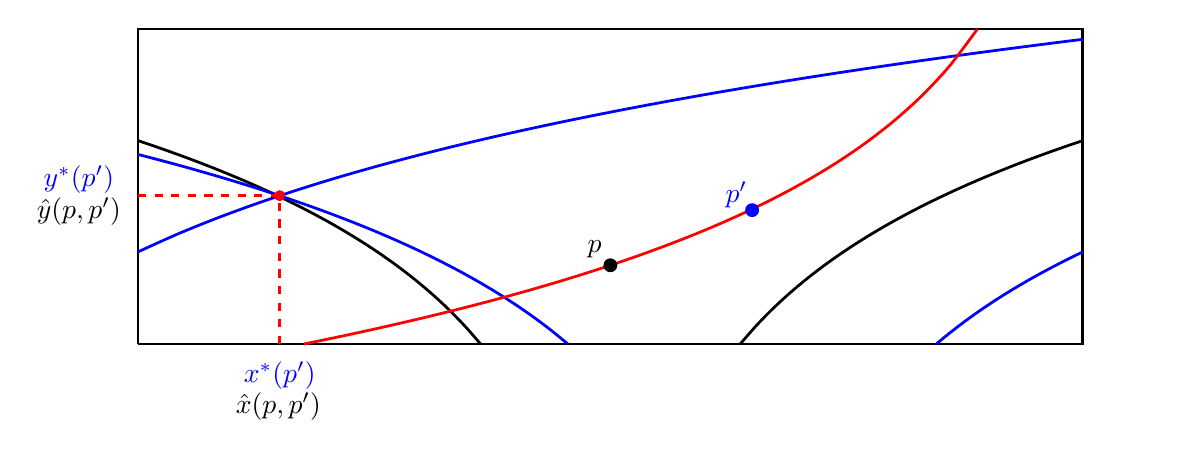
\begin{tikzpicture}
	%Define the coordinates 
	%p = (\u,\v) and p^\prime = (\uu, \vv)
	%Box \Rcal_n has width 2\r and height \t
	\pgfmathsetmacro{\u}{0}
	\pgfmathsetmacro{\v}{1}
	\pgfmathsetmacro{\uu}{1.8}
	\pgfmathsetmacro{\vv}{1.7}
	\pgfmathsetmacro{\r}{6}
	\pgfmathsetmacro{\t}{4}
	
	%The box \Rcal_n
	\draw[line width=1pt] (-\r,0) -- (\r,0) -- (\r,\t) -- (-\r,\t) -- (-\r,0);	
	
	%Boundaries p = (\u,\v)
	
	%Right boundary
	\pgfmathsetmacro{\rightbounduv}{\u+exp((\v)/2)}
	\draw[domain=\rightbounduv:\r,smooth,variable=\x,black,line width=1pt] plot (\x, {2*ln(\x)-\v});
    %Left boundary
    \pgfmathsetmacro{\leftbounduv}{\u-exp((\v)/2)}
    \draw[domain=\leftbounduv:-\r,smooth,variable=\x,black,line width=1pt] plot (\x, {2*ln(-\x)-\v});
    
    %Boundaries p^\prime = (\uu,\vv)
    
    %Right boundary
    \pgfmathsetmacro{\rightbounduuvv}{\uu+exp((\vv)/2)}
    \draw[domain=\rightbounduuvv:\r,smooth,variable=\x,blue,line width=1pt] plot (\x, {2*ln(\x-\uu)-\vv});
    %Shifted right boundary
    \pgfmathsetmacro{\shiftrightbounduuvv}{\uu+exp((\vv + \t)/2)-2*\r}
    %\draw[domain=\shiftrightbounduuvv:-\r,smooth,variable=\x,blue,line width=1pt] plot (\x, {2*ln(\x+(2*\r-\uu))-\vv});
    \draw[domain=-\r:\r,smooth,variable=\x,blue,line width=1pt] plot (\x, {2*ln(\x+(2*\r-\uu))-\vv});
    %Left boundary 
    \pgfmathsetmacro{\leftbounduuvv}{\uu-exp((\vv)/2)}
    \draw[domain=\leftbounduuvv:-\r,smooth,variable=\x,blue,line width=1pt] plot (\x, {2*ln(\uu-\x)-\vv});
    %Shifted left boundary

    
    %Star boundary
    \pgfmathsetmacro{\starleftbound}{\r*(1-exp(\v/2))}
    \pgfmathsetmacro{\starrightbound}{\r*(1-exp((\v-\t)/2))}
    \draw[domain=\starleftbound:\starrightbound,smooth,variable=\x,red, line width=1pt] plot (\x, {2*ln((\r/(\r-\x)))+\v});
    
    %Define h_1(p) = h_2(p)
    \pgfmathsetmacro{\hp}{2*ln(\r-\u)-\v}
%    \draw node at (\r+0.75,\hp) {\color{black}$h(y)$};
    \draw node at (\r+1,\hp) {};
    
    %Define h_1(p^\prime) and h_2(p^\prime)
    \pgfmathsetmacro{\hh}{2*ln(\uu+\r)-\vv}
    \pgfmathsetmacro{\hhh}{2*ln(\r-\uu)-\vv}

%    \draw node at (-\r-0.75,\hh+0.1) {\color{blue}$h_1(p^\prime)$};
%    \draw node at (\r+0.75,\hhh) {\color{blue}$h_2(p^\prime)$};
    
    %Define x^\ast(p^\prime) and y^\ast(p^\prime), intersection of left and shifted right blue curve
    \pgfmathsetmacro{\uuast}{\uu-\r}
    \pgfmathsetmacro{\vvast}{2*ln(\r)-\vv}

    %Define intersection left black and shifted blue curve
    \pgfmathsetmacro{\vast}{2*ln((2*\r - \uu)/(exp(\v/2) + exp(\vv/2)))}
    \pgfmathsetmacro{\uast}{(\uu - 2*\r)/(1 + exp((\vv - \v)/2))} 

%    \draw[dashed,thick,black] (-\r,\hhh) -- (\r,\hhh);
    \draw[dashed,line width=1pt,red] (\uuast,0) -- (\uuast,\vvast);
    \draw node at (\uuast,-0.4) {\color{blue}$x^\ast(p^\prime)$};
    \draw[dashed,line width=1pt,red] (-\r,\vvast) -- (\uuast,\vvast);
    \draw node at (-\r-0.75,\vvast+0.2) {\color{blue}$y^\ast(p^\prime)$};
%    \draw[dashed,black,line width=1pt] (-\r,\vast) -- (\uast,\vast);
    \draw node at (-\r-0.75,\vast-0.2) {\color{black}$\hat{y}(p,p^\prime)$};
%    \draw[dashed,black,line width=1pt] (\uast,\vast) -- (\uast,0);
    \draw node at (\uast,-0.8) {\color{black}$\hat{x}(p,p^\prime)$};
    
    \draw node[fill, circle, inner sep=0pt, minimum size=4pt, red] at (\uuast,\vvast) {};
    
   	%Draw both nodes
    \draw node[fill, circle, inner sep=0pt, minimum size=5pt] (p1) at (\u,\v) {};
    \path (p1)+(-0.2,0.2) node {$p$};
    \draw node[fill,blue, circle, inner sep=0pt, minimum size=5pt] (p2) at (\uu,\vv) {};
    \path (p2)+(-0.2,0.2) node {\color{blue}$p^\prime$};
    
    
    
%    \draw node[fill, circle, inner sep=0pt, minimum size=4pt, black] at (\uast,\vast) {};
    
%    \draw node at (-7,2.5835) {$h(y)$};

    
%    \draw[dotted,thick,black] (4.5208,2.0174) -- (4.5208,0);
%    \draw[dotted,thick,black] (4.5208,2.0174) -- (6,2.0174);
    
%    \draw node at (4.5208,-0.5) {$w_x(p,p^\prime)$};
%    \draw node at (7,2.0174) {$w_y(p,p^\prime)$};
    
%    \draw node at (0,3.5) {\color{blue}$x_1 = x^\prime + e^{\frac{y^\prime + y_1}{2}}$};
%    \draw node at (-2,1.6) {\color{blue}$x_1 = x^\prime - e^{\frac{y^\prime + y_1}{2}}$};
%    \draw node at (-4.5,1) {$x_1 = x - e^{\frac{y + y_1}{2}}$};
%    \draw node at (2,1.5) {$x_1 = x + e^{\frac{y + y_1}{2}}$};

\end{tikzpicture}
\caption{???.}
\label{fig:comparing_triangles_diff_analysis}
\end{figure}

This analysis allows us to compute the expected difference in the number of triangles for $\Pcal$ and $\Pcal_n$, for a node with height $y$. 

\begin{lemma}\label{lem:clustering_error_T_term}
Let $(k_n)_{n \ge 1}$ be any sequence with $k_n \to \infty$ and $k_n = \smallO{n^{\frac{1}{2\alpha + 1}}}$. Then, for any $0 < \varepsilon < 1$ and $p \in \Kcal_{\varepsilon}(k_n)$, as $n \to \infty$,
\[
	\int_{\Rcal_n} \mu_{\alpha, \nu}\left(\mathcal{T}_{\Pcal \Delta \Pcal_n}(p,p_1)\right) f_{\mu, \nu}(x_1,y_1) 
	\dd x_1 \dd y_1 = \bigO{y n^{-(2\alpha - 1)} + n^{-(2\alpha-1)} e^{y}}
\]
\end{lemma}

The proof of the lemma is not difficult but cumbersome, since it involves computing many different integrals. We postpone this proof till the end of this section and proceed with the main goal, proving Proposition~\ref{prop:convergence_average_clustering_P_n}. But first we state a small lemma about the scaling of $s_\alpha(k_n)$ that will be very useful.  

\begin{lemma}\label{lem:scaling_s_alpha}
Let $s_\alpha(k_n)$ be as defined in \eqref{eq:def_scaling_function}. Then for any $k_n = \smallO{n^{\frac{1}{2\alpha + 1}}}$, as $n \to \infty$,
\[
	n^{-(2\alpha - 1)} = \smallO{s_\alpha(k_n)}.
\]
\end{lemma}

\begin{proof}
First let $\frac{1}{2} < \alpha < \frac{3}{4}$. Then
\[
	n^{-(2\alpha - 1)}s_\alpha(k_n)^{-1} = n^{-(2\alpha -1)}k_n^{4\alpha - 2}
	= \smallO{n^{-(2\alpha - 1) + \frac{4\alpha - 2}{2\alpha + 1}}} 
	= \smallO{n^{-\frac{4\alpha^2 - 4\alpha + 1}{2\alpha + 1}}}
	= \smallO{1},
\]
since $4\alpha^2 - 4\alpha + 1 > 0$ for all $\alpha > \frac{1}{2}$. Similarly, for $\alpha \ge \frac{3}{4}$ we have
that $4\alpha^2 > 2$ and hence,
\[
	n^{-(2\alpha - 1)} s_{\alpha}(k_n) = \smallO{n^{-(2\alpha - 1)} k_n} = \smallO{n^{-\frac{4\alpha^2 - 2}{2\alpha + 1}}}
	= \smallO{1}.
\]
\end{proof}

\begin{corollary}\label{cor:clustering_error_T_term}
Let $(k_n)_{n \ge 1}$ be any sequence with $k_n \to \infty$ and $k_n = \smallO{n^{\frac{1}{2\alpha + 1}}}$. Then, for any $0 < \varepsilon < 1$ and $p \in \Kcal_{\varepsilon}(k_n)$, as $n \to \infty$,
\[
	\left|\frac{\Exp{T_{\Pcal,n}(p)}}{\Exp{T_{\Pcal}(p)}} - 1\right| = \bigO{s_\alpha(k_n)^{-1} k_n^{-3(2\alpha - 1)}} =
	\begin{cases}
		\bigO{k_n^{-(2\alpha - 1)}} &\mbox{if } \frac{1}{2} < \alpha < \frac{3}{4},\\
				\bigO{\log(k_n)^{-1} k_n^{-\frac{1}{2}}} &\mbox{if } \alpha = \frac{3}{4},\\
				\bigO{k_n^{-(6\alpha-4)}} &\mbox{if } \alpha > \frac{3}{4}.
	\end{cases}
\]
\end{corollary}

\begin{proof}[Proof of Proposition~\ref{prop:convergence_average_clustering_P_n}]

\PvdH{incorporate case where $k_n = \bigT{1}$.}

Recall that
\[
	\Exp{c_{\Pcal,n}^\ast(k_n)} = \frac{\int_{\Rcal_n} \rho_n(y,k_n) \Exp{T_{\Pcal,n}(y)} f_{\alpha,\nu}(x,y) \dd x \dd y}{\binom{k_n}{2}\Exp{N_{\Pcal,n}(k_n)}}.
\]
By Lemma~\ref{lem:nodes_degree_k_P_n}
\[
	\Exp{N_{\Pcal,n}(k_n)} = (1+o(1)) \alpha n \int_{\R_+} \rho(y,k_n) e^{-\alpha} \dd y,
\]
and hence it is enough to show that
\[
	\int_{\Rcal_n} \rho_n(y,k_n) \Exp{T_{\Pcal,n}(y)} f_{\alpha,\nu}(x,y) \dd x \dd y
	= (1 + \smallO{1}) \alpha n \int_{\R_+} \rho(y,k_n) \Exp{T_\Pcal(y)} e^{-\alpha y} \dd x \dd y.
\]

First we note that
\begin{align*}
	\left|T_{\Pcal,n}(p) - T_{\Pcal}(p)\right| = \sum_{p_1, p_2 \in \Rcal_n} \ind{p_1 \in \BallPon{p}} \ind{p_2 \in \mathcal{T}_{\Pcal \Delta \Pcal_n}(p, p_1)} + \sum_{p_1, p_2 \in \Rcal \setminus \Rcal_n} T_{\Pcal}(p,p_1,p_2)
\end{align*}
and hence
\begin{align*}
	\left|\Exp{T_{\Pcal,n}(p) - T_{\Pcal}(p)}\right|
	&\le \int_{\Rcal_n} \mu_{\alpha, \nu}\left(\mathcal{T}_{\Pcal \Delta \Pcal_n}(p,p_1)\right) f_{\mu, \nu}(x_1,y_1) 
		\dd x_1 \dd y_1\\
	&\hspace{10pt}+ \iint_{\Rcal \setminus \Rcal_n} T_{\Pcal}(p,p_1,p_2) f_{\mu, \nu}(x_1,y_1) f_{\mu, \nu}(x_2,y_2)
		\dd x_2 \dd y_2 \dd x_1 \dd y_1. 
\end{align*}

The first integral was taken care of in Lemma \ref{lem:clustering_error_T_term}. For the second integral we have
\begin{align*}
	&\hspace{-30pt}\iint_{\Rcal \setminus \Rcal_n} T_{\Pcal}(p,p_1,p_2) f_{\mu, \nu}(x_1,y_1) f_{\mu, \nu}(x_2,y_2)
		\dd x_2 \dd y_2 \dd x_1 \dd y_1\\
	&\le \left(\int_{\Rcal \setminus \Rcal_n} \ind{p_1 \in \BallPo{p}} f_{\mu, \nu}(x_1,y_1) \dd x_1 \dd y_1\right)^2\\
	&= \bigO{\left(e^{y/2} \int_{R_n}^\infty e^{-(\alpha - \frac{1}{2})y_1} \dd y_1\right)^2}
		= \bigO{e^y n^{-(2\alpha - 1)}},
\end{align*}
from which we conclude that
\[
	\left|\Exp{T_{\Pcal,n}(p) - T_{\Pcal}(p)}\right| = \bigO{y n^{-(2\alpha - 1)} + n^{-(2\alpha-1)} e^{y}}
	= \bigO{n^{-(2\alpha-1)} e^{y}}.
\]
Next we show that this difference is $\smallO{\Exp{T_\Pcal(p)}}$ when $y \in K_\eps(k_n)$.
Observe that since $\Exp{T_\Pcal(p)} = e^y \Delta_{\Pcal}(y)$, Proposition~\ref{prop:asymptotics_Delta_y_P} implies that $\Exp{T_\Pcal(y)} = \bigT{e^y s_\alpha(e^{y/2})}$ as $y \to \infty$.
Now consider $y \in K_C(k_n)$. Then $e^{y/2} = \bigT{k_n}$ and hence
\[
	\frac{\left|\Exp{T_{\Pcal,n}(p) - T_{\Pcal}(p)}\right|}{\Exp{T_\Pcal(y)}} =
	\bigO{n^{-(2\alpha - 1)}s_\alpha(k_n)^{-1}\left(\log(k_n)k^{-2} + 1\right)} = \bigO{\left(n^{2\alpha - 1}s_\alpha(k_n)\right)^{-1}} = \smallO{1}, 
\]
where the last part follows from Lemma~\ref{lem:scaling_s_alpha}. It follows that for $y \in \Kcal_\eps(k_n)$ we have
\[
	\Exp{T_{\Pcal,n}(y)} = (1+\smallO{1})\Exp{T_{\Pcal}(y)},
\]
while in general
\[
	\Exp{T_{\Pcal,n}(y)} = \Exp{T_{\Pcal}(y)}\left(1 + \bigO{s_\alpha(e^{y/2})}\right) = \bigO{e^y s_\alpha(e^{y/2})^2}.
\]
Therefore, by first applying a concentration argument and then Lemma~\ref{lem:replace_rho_n_with_rho}, 
\begin{align*}
	&\hspace{-30pt}\int_{\Rcal_n} \rho_n(y,k_n) \Exp{T_{\Pcal,n}(y)} f_{\alpha,\nu}(x,y) \dd x \dd y\\
	&= (1+\smallO{1})\int_{\Rcal_n} \rho_n(y,k_n) \Exp{T_\Pcal(y)} f_{\alpha,\nu}(x,y) \dd x \dd y\\
	&= (1 + \smallO{1}) \int_{\Rcal_n} \rho(y,k_n) \Exp{T_\Pcal(y)} f_{\alpha,\nu}(x,y) \dd x \dd y\\
	&= (1 + \smallO{1}) \alpha n \int_{\R_+} \rho(y,k_n) \Exp{T_\Pcal(y)} e^{-\alpha y} \dd x \dd y.
\end{align*}
\end{proof}

%\begin{corollary}
%\[
%	\Exp{T_{\Pcal,n}(k_n)} = \begin{cases}
%		\bigT{n k_n^{-3(2\alpha - 1)}} &\mbox{if } \frac{1}{2} < \alpha < \frac{3}{4}\\
%		\bigT{n \log(k_n) k^{-2\alpha}} &\mbox{if } \alpha = \frac{3}{4} \\
%		\bigT{n k^{-2\alpha}} &\mbox{if } \alpha > \frac{3}{4}.
%	\end{cases}
%\]
%\end{corollary}
%
%\begin{remark}
%Note that for $p_0 \notin \Kcal_\varepsilon(k_n)$, we could have proven that
%\[
%	\left|\Delta_{\Pcal, n}(y) - \Delta_{\Pcal}(y)\right| = \bigO{n^{-\lambda}e^{(\alpha -\frac{1}{2})y}},
%\]
%for some $\lambda > 0$. However, this would have required us to do a more thorough analysis of the integral
%\[
%	\int_{\mathcal{E}_n} \Delta(p_0,p_1,p_2)g_{p_0}(x_1,y_1) g_{p_0}(x_2,y_2) \, dx_2 \, dx_1 \, dy_2 \, dy_1,
%\]
%making the proof more cumbersome. Since for our purpose we only need the $e^{\beta y}$ term, we omitted this additional analysis.
%\end{remark}

%\subsection{Equivalence for local clustering in $G_{\Pcal}(\alpha, \nu)$ and $G_{\Pcal,n}(\alpha,\nu)$}
%
%We now proceed with the proof of Proposition \ref{prop:convergence_average_clustering_P_n}. For this we split 
%$\left|\Exp{c_{\Pcal,n}^\ast(k_n)} - \Exp{c_{\Pcal}^\ast(k_n)}\right|$ into three different terms which each evaluate the difference between the different elements of the local clustering function. We then analyze each term separately. The main tool we use is Lemma \ref{lem:clustering_error_Delta_term} together with the splitting technique we used in the proof of Lemma \ref{lem:asymptotics_integral_outside_K_epsilon}, which considers the integral over $\Kcal_\varepsilon(k_n)$ and $\Rcal_n \setminus \Kcal_\varepsilon(k_n)$ separately. 
%
%\begin{lemma}
%\[
%	\lim_{n \to \infty} \frac{\Exp{\widetilde{T}_{\Pcal,n}(k,\varepsilon)}}{\Exp{T_{\Pcal}(k)}} = 1.
%\]
%\end{lemma}
%
%\begin{proof}[Proof of Proposition \ref{prop:convergence_average_clustering_P_n}]
%
%We give the proof for the case $\frac{1}{2} < \alpha < \frac{3}{4}$. The proof for the other cases are similar.
%
%Let $0 < \varepsilon < 1$ and recall the definition $a_n^\pm = 2\log\left(\frac{(1\pm\varepsilon)k_n}{2\xi_{\alpha,\nu}}\right)$. In addition, recall that
%\[
%	\Exp{c_{\Pcal,n}^\ast(k_n)} = \int_{\Rcal_n} \frac{\Delta_{\Pcal,n}(y) \rho_k(y)}{\Exp{N_{\Pcal,n}(k_n)} \binom{k_n}{2}}  
%    f_{\alpha, \nu}(x,y) \, dx \, dy.
%\]
%
%We now use Lemma \ref{lem:expectation_clustering_P} and \eqref{eq:expectation_clustering_P_n} to write
%\begin{align*}
%	\left|\Exp{c_{\Pcal,n}^\ast(k_n) - c_{\Pcal}^\ast(k_n)}\right|
%	&= \left|\frac{\int_0^{R_n} \Delta_{\Pcal,n}(y) \, \rho_{n,y}(k_n) e^{-\alpha y} \, dy}
%		{\int_0^{R_n} \rho_{n,y}(k_n) e^{-\alpha y} \, dy} 
%		- \frac{\int_0^{\infty} \Delta_{\Pcal}(y) \, \rho_{y}(k_n) e^{-\alpha y} \, dy}
%		{\int_0^{\infty} \rho_{y}(k_n) e^{-\alpha y} \, dy}\right|\\
%	&\le \frac{\int_0^{R_n} \left|\Delta_{\Pcal,n}(y) \, \rho_{n,y}(k) - \Delta_{\Pcal}(y) \, \rho_{y}(k)\right| 
%		e^{-\alpha y} \, dy}{\int_0^{\infty} \rho_{y}(k) e^{-\alpha y} \, dy} \\
%	&\hspace{10pt}+ \frac{\int_{R_n}^\infty \Delta_{\Pcal}(y) \, \rho_{y}(k) 
%			e^{-\alpha y} \, dy}{\int_0^{\infty} \rho_{y}(k) e^{-\alpha y} \, dy}\\
%	&\hspace{10pt}+ \frac{\int_0^{R_n} \Delta_{\Pcal,n}(y) \, \rho_{n,y}(k) e^{-\alpha y} \, dy}
%		{\int_0^{R_n}  \rho_{y}(k_n) e^{-\alpha y} \, dy}
%		\left|\frac{\int_0^{R_n}  \rho_{y}(k_n) e^{-\alpha y} \, dy}{\int_0^{\infty} \rho_{n,y}(k_n) e^{-\alpha y} \, dy}
%		- 1\right|\\
%	&:= I_n^{(1)}(k_n) + I_n^{(2)}(k_n) + I_n^{(3)}(k_n)
%\end{align*}
%We will deal with all three terms separately and show that
%\begin{equation}
%	\lim_{n \to \infty} k_n^{4\alpha - 2} I_n^{(i)}(k_n) = 0 \quad \text{for } i = 1, 2, 3.
%\end{equation} 
%
%For $I_n^{(1)}(k_n)$ we write
%\begin{align}
%	I_n^{(1)}(k_n)	&\le \frac{\int_0^{R_n} \left|\Delta_{\Pcal,n}(y)  - \Delta_{\Pcal}(y) \right| \rho_{y}(k_n)
%		e^{-\alpha y} \, dy}{\int_0^{\infty} \rho_{y}(k_n) e^{-\alpha y} \, dy} 
%        \label{eq:diff_Delta_integral}\\
%	&\hspace{10pt}+ \frac{\int_0^{R_n} \left|\rho_{n, y}(k) - \rho_{y}(k_n)\right| \Delta_{\Pcal,n}(y) 
%		e^{-\alpha y} \, dy}{\int_0^{\infty} \rho_{y}(k_n) e^{-\alpha y} \, dy}. \label{eq:diff_Poisson_distribution}
%\end{align}
%
%For \eqref{eq:diff_Delta_integral} we use Lemma \ref{lem:clustering_error_Delta_term} to obtain
%\begin{align*}
%	\int_0^{R_n} \left|\Delta_{\Pcal,n}(y)  - \Delta_{\Pcal}(y) \right| \rho_{y}(k_n) e^{-\alpha y} \, dy
%    &\le \bigO{k_n^{-3(2\alpha - 1)}}\int_{a_n^-}^{a_n^+} \rho_{y}(k_n) e^{-\alpha y} \, dy\\
%    &\hspace{10pt}+ \bigO{n^{-(2\alpha - 1)}k^{2\alpha - 1}\int_0^\infty \Delta_\Pcal(y)\rho_{y}(k_n) e^{-\alpha y} 
%    	\, dy}\\
%    &\hspace{10pt}+ \bigO{\frac{1}{n}\int_{\Rcal_n \setminus \Kcal_\varepsilon(k_n)} e^{(\alpha - \frac{1}{2})y} 
%    	\rho_{y}(k_n) f_{\alpha,\nu}(x,y) \, dx \, dy}.
%\end{align*}
%Observe that first term is bounded from above by
%\[
%	\bigO{k_n^{-3(2\alpha - 1)}} \int_0^\infty \rho_y(k_n) e^{-\alpha y} \, dy
%\]
%and recall that $\int_0^{\infty} \rho_{y}(k_n) e^{-\alpha y} \, dy = \Theta\left(k_n^{-(2\alpha + 1)}\right)$. Hence
%\begin{align*}
%	&\hspace{-30pt}k_n^{4\alpha - 2} \, \frac{\int_0^{R_n} \left|\Delta_{\Pcal,n}(y) - \Delta_{\Pcal}(y) 
%		\right| \rho_{y}(k_n) e^{-\alpha y} \, dy}{\int_0^{\infty} \rho_{y}(k) e^{-\alpha y} \, dy}\\
%    &= \bigO{k_n^{4\alpha - 2} k_n^{-3(2\alpha - 1)}} + \bigO{n^{-(2\alpha - 1)}k^{2\alpha - 1}} k_n^{4\alpha - 2}\Exp{c_\Pcal^\ast(k_n)}\\
%	&\hspace{10pt}+ \bigO{k_n^{6\alpha - 1} \frac{1}{n}\int_{\Rcal_n \setminus \Kcal_\varepsilon(k_n)} e^{(\alpha - \frac{1}{2})y} 
%    	\rho_{y}(k_n) f_{\alpha,\nu}(x,y) \, dx \, dy}.
%\end{align*}
%The first term here is $\bigO{k_n^{-(\alpha - \frac{1}{2})}}$ which converges to zero. The second term converges to zero by [Proposition on scaling] and the fact that $n^{-(2\alpha - 1)}k^{2\alpha - 1} = o(1)$. The same holds for the third term by Lemma \ref{lem:asymptotics_integral_outside_K_epsilon}. 
%
%For \eqref{eq:diff_Poisson_distribution} we apply the same splitting technique as in the proof of Lemma \ref{lem:clustering_error_Delta_term}. That is, we take $0 < \varepsilon < 1$, $a_n^+ = 2\log\left((1+\varepsilon)k_n\right)$ and write
%\begin{align*}
%	\int_0^{R_n} \left|\rho_{n, y}(k) - \rho_{y}(k_n)\right| \Delta_{\mu_n}(y) e^{-\alpha y} \, dy
%	&= \int_0^{a_n^+} \left|\rho_{n, y}(k) - \rho_{y}(k_n)\right| \Delta_{\mu_n}(y) e^{-\alpha y} \, dy\\
%	&\hspace{10pt}+ \int_{a_n^+}^{R_n} \left|\rho_{n, y}(k) - \rho_{y}(k_n)\right| \Delta_{\mu_n}(y) e^{-\alpha y} \, dy
%\end{align*}
%Next we use Lemma \ref{lem:mu_measure_B} to obtain
%\begin{align*}
%	\rho_{n, y}(k_n) &= \rho_y(k_n) \left((1+\phi_n(y))^{k_n} \left(1 - e^{-\alpha R_n}\right)^{-k_n}
%		e^{-\mu(B(0,y))\left(\phi_n(y) + \frac{(1 + \phi_n(y))e^{-\alpha R_n}}{1 - e^{-\alpha R_n}}\right)}\right).
%\end{align*}
%Using that
%\begin{align*}
%	\max_{0 \le y \le a_n} \hspace{-5pt} \phi_n(y)
%	= O\left(n^{-(2\alpha - 1)(1-\kappa)}\right) \quad \text{and} \quad
%	\int_0^{\infty} \rho_{y}(k_n) e^{-\alpha y} \, dy = \Theta\left(k_n^{-(2\alpha + 1)}\right)
%\end{align*}
%we get for the first integral,
%\begin{align*}
%	&\hspace{-30pt}k_n^{4\alpha - 2}\frac{\int_0^{a_n} \left|\rho_{n, y}(k) - \rho_{y}(k_n)\right| \Delta_{\mu_n}(y) 
%		e^{-\alpha y} \, dy}{\int_0^{\infty} \rho_{y}(k_n) e^{-\alpha y} \, dy}\\
%	&= O\left(n^{-(2\alpha - 1)(1-\kappa)} k_n^{4\alpha - 2}\frac{\int_0^\infty \Delta_{\mu}(y) \rho_{y}(k_n) e^{-\alpha y} 
%		\, dy}{\int_0^{\infty} \rho_{y}(k_n) e^{-\alpha y} \, dy}\right)\\
%	&= O\left(n^{-(2\alpha - 1)(1-\kappa)}\right).
%\end{align*}
%For the second integral we use that $\phi_n(y) = O(1)$ for all $0 \le y \le R_n$ and hence, using the same argumentation as at the end of the proof of Lemma \ref{lem:clustering_error_Delta_term},
%\begin{align*}
%	&\hspace{-30pt}k_n^{4\alpha - 2}\frac{\int_{a_n}^{R_n} \left|\rho_{n, y}(k) - \rho_{y}(k_n)\right| \Delta_{\mu_n}(y) 
%		e^{-\alpha y} \, dy}{\int_0^\infty \rho_y(k_n) \, e^{-\alpha y} \, dy}\\
%	&= O\left(k_n^{4\alpha - 2}\frac{\int_{a_n}^{R_n} \rho_{y}(k_n) \Delta_{\mu}(y) e^{-\alpha y} \, dy}
%		{\int_0^\infty \rho_y(k_n) \, e^{-\alpha y} \, dy}\right)\\
%	&= O\left(k_n^{6\alpha - 1}\rho_{a_n}(k_n)\right) = o(1).
%\end{align*}
%We therefore conclude that $k_n^{4\alpha - 2}I_n^{(1)}(k_n) \to 0$.
%
%Next we consider the second term
%\[
%	I_n^{(2)}(k_n) = \frac{\int_{R_n}^\infty \Delta_{\mu}(y) \, \rho_{y}(k) 
%		e^{-\alpha y} \, dy}{\int_0^{\infty} \rho_{y}(k) e^{-\alpha y} \, dy}.
%\]
%Since
%\[
%	\int_{R_n}^\infty \Delta_{\mu}(y) \, \rho_{y}(k) e^{-\alpha y} \, dy 
%	\le \rho_{R_n}(k_n) \int_0^\infty e^{-\alpha y} \, dy = O\left(\rho_(R_n)(k_n)\right) 
%	= O\left(\rho_{a_n}(k_n)\right),
%\]
%it follows from the above computations that
%\[
%	\lim_{n \to \infty} k_n^{4\alpha - 2} \frac{\int_{R_n}^\infty \Delta_{\mu}(y) \, \rho_{y}(k) 
%	e^{-\alpha y} \, dy}{\int_0^{\infty} \rho_{y}(k) e^{-\alpha y} \, dy} = 0.
%\]
%The proof for $I_n^{(3)}(k_n)$ follows using the same splitting technique and arguments. We therefore omit it.
%\end{proof}

\subsection{Counting missing triangles}

We now come back to computing the expected number of triangles attached to node at height $y$ in $G_{\Pcal,n}(\alpha,\nu)$ that are not present in $G_{\Pcal}(\alpha,\nu)$. 

\begin{figure}[!t]

\centering
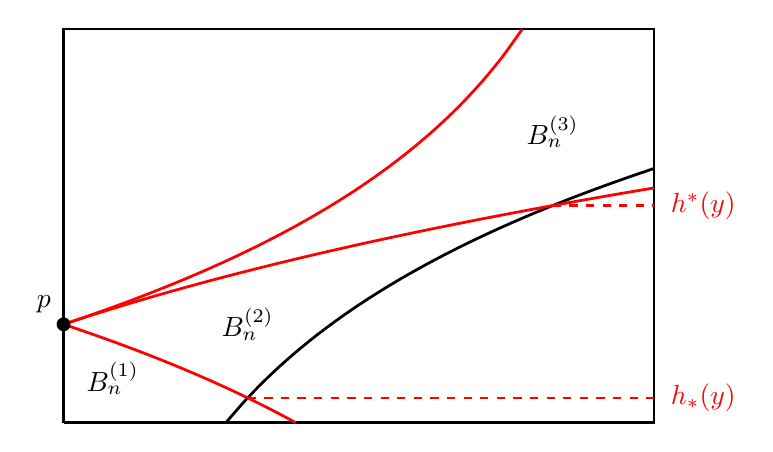
\begin{tikzpicture}[scale=1.25]

%%%%%%%%%%%%%%%%%%%%%%%%%%%%%%%%%%%%%%%%%%%%%%%%%%%%%%%%%%%%%%%%%%%%%%%%%%%%%%%%%%%%%%%%%%%%%%%%%%%
%																								  %
%	Shows the three different areas B_n^{(i)} for the computations in Lemma 					  %
%	\label{lem:clustering_error_T_term}			  												  %
%																								  %
%%%%%%%%%%%%%%%%%%%%%%%%%%%%%%%%%%%%%%%%%%%%%%%%%%%%%%%%%%%%%%%%%%%%%%%%%%%%%%%%%%%%%%%%%%%%%%%%%%%

	%Define the coordinates 
	%p = (\u,\v) and p^\prime = (\uu, \vv)
	%Box \Rcal_n has width 2\r and height \t
	\pgfmathsetmacro{\u}{0}
	\pgfmathsetmacro{\v}{1}
	\pgfmathsetmacro{\uu}{1.8}
	\pgfmathsetmacro{\vv}{1.7}
	\pgfmathsetmacro{\r}{6}
	\pgfmathsetmacro{\t}{4}
	
	%The box \Rcal_n only positive x
	\draw[line width=1pt] (0,0) -- (\r,0) -- (\r,\t) -- (0,\t) -- (0,0);	
	
	%Boundaries p = (\u,\v)
	
	%Right boundary
	\pgfmathsetmacro{\rightbounduv}{\u+exp((\v)/2)}
	\draw[domain=\rightbounduv:\r,smooth,variable=\x,black,line width=1pt] plot (\x, {2*ln(\x)-\v});
    %Left boundary
%    \pgfmathsetmacro{\leftbounduv}{\u-exp((\v)/2)}
%    \draw[domain=\leftbounduv:-\r,smooth,variable=\x,black,line width=1pt] plot (\x, {2*ln(-\x)-\v});
    
    %Three boundaries for the regions B_n
    \pgfmathsetmacro{\bone}{\r*(1-exp(-\v/2))}
    \pgfmathsetmacro{\btwo}{\r*(exp(-\v/2)-1)}
    %Star boundary
    \pgfmathsetmacro{\bthreeleft}{\r*(1-exp(\v/2))}
    \pgfmathsetmacro{\bthreeright}{\r*(1-exp((\v-\t)/2))}
    
    \draw[domain=0:\bone,smooth,variable=\x,red,line width=1pt] plot (\x, {\v-2*ln(\r/(\r-\x))});
    \draw[domain=0:\r,smooth,variable=\x,red,line width=1pt] plot (\x, {\v+2*ln(1+(\x/\r))});
    \draw[domain=0:\bthreeright,smooth,variable=\x,red, line width=1pt] plot (\x, {2*ln((\r/(\r-\x)))+\v});    
    
    %Define the top and bottom coordinates of y^prime boundaries
    \pgfmathsetmacro{\ybottom}{\v+2*ln(\r/(\r+exp(\v)))}
    \pgfmathsetmacro{\xbottom}{\r*exp(\v)/(\r + exp(\v))}
    \pgfmathsetmacro{\ytop}{\v+2*ln(\r/(\r-exp(\v)))}
    \pgfmathsetmacro{\xtop}{\r*exp(\v)/(\r - exp(\v))}
    
    \draw[dashed,line width=1pt,red] (\xbottom,\ybottom) -- (\r,\ybottom);
    \draw[dashed,line width=1pt,red] (\xtop,\ytop) -- (\r,\ytop);
    \draw node at (\r+0.5,\ybottom) {\color{red}$h_\ast(y)$};
    \draw node at (\r+0.5,\ytop) {\color{red}$h^\ast(y)$};
    
    \draw node at (0.5,\ybottom+0.2) {$B_n^{(1)}$};
    \draw node at (\xbottom,\ybottom+0.75) {$B_n^{(2)}$};
    \draw node at (\xtop,\ytop+0.75) {$B_n^{(3)}$};
    

    %Define h_1(p) = h_2(p)
    \pgfmathsetmacro{\hp}{2*ln(\r-\u)-\v}
  
    %Define h_1(p^\prime) and h_2(p^\prime)
    \pgfmathsetmacro{\hh}{2*ln(\uu+\r)-\vv}
    \pgfmathsetmacro{\hhh}{2*ln(\r-\uu)-\vv}

%    \draw node at (-\r-0.75,\hh+0.1) {\color{blue}$h_1(p^\prime)$};
%    \draw node at (\r+0.75,\hhh) {\color{blue}$h_2(p^\prime)$}; 
    
   	%Draw node p
    \draw node[fill, circle, inner sep=0pt, minimum size=5pt] (p1) at (\u,\v) {};
    \path (p1)+(-0.2,0.2) node {$p$};

\end{tikzpicture}
\caption{Three different areas $B_n^{(i)}$ used in the proof of Lemma \ref{lem:clustering_error_T_term}.}
\label{fig:comparing_triangles_B_areas}
\end{figure}

\begin{proof}[Proof of Lemma \ref{lem:clustering_error_T_term}]
Due to symmetry it is enough to show that
\begin{equation}\label{eq:clustering_error_T_main}
	\int_0^{R_n}\int_0^{I_n} \mu_{\alpha, \nu}\left(\mathcal{T}_{\Pcal \Delta \Pcal_n}(p,p_1)\right) f_{\mu, \nu}(x_1,y_1) 
	\dd x_1 \dd y_1 = \bigO{y n^{-(2\alpha - 1)} + n^{-(2\alpha-1)} e^{y}}
\end{equation}
The proof goes in two stages. First we compute $\mu_{\alpha, \nu}\left(\mathcal{T}_{\Pcal \Delta \Pcal_n}(p,p_1)\right)$ by splitting it over three disjoint regimes with respect to $p_1$, with $x_1 \ge 0$. Then we do the integration with respect to $p_1$.

\subsubsection*{Computing $\bm{\mu_{\alpha, \nu}\left(\mathcal{T}_{\Pcal \Delta \Pcal_n}(p,p_1)\right)}$}

\PvdH{I have currently used that $\alpha < 1$, which is the most difficult case. The case $\alpha = 1$ and $\alpha > 1$ will be added.}

Define the sets
\begin{align*}
	A_n^{(1)} &= \left\{p_1 \in \Rcal_n \, : \, 0 \le y_1 \le y - 2\log(I_n/(I_n-x_1)) \right\},\\
	A_n^{(2)} &= \left\{p_1 \in \Rcal_n \, : \, y - 2\log(I_n/(I_n-x_1)) < y_1 
		\le y + 2 \log\left(1 + \frac{x_1}{I_n}\right)\right\},\\
	A_n^{(3)} &= \left\{p_1 \in \Rcal_n \, : \, y + 2 \log\left(1 + \frac{x_1}{I_n}\right) < y_1 
			\le y + 2 \log\left(\frac{I_n}{I_n-x_1}\right)\right\},
\end{align*}
and let $B_n^{(i)} = \BallPon{p} \cap A_n^{(i)}$, for $i = 1, 2, 3$, see Figure~\ref{fig:comparing_triangles_B_areas}. Here the heights of the two intersections are given by
\begin{align}
	h_\ast(y) &= y + 2 \log\left(\frac{I_n}{I_n + e^y}\right)\\
	h^\ast(y) &= y + 2 \log\left(\frac{I_n}{I_n - e^y}\right).
\end{align}

With these definitions we have that the union $B_n := \bigcup_{i = 1}^n B_n^{(i)}$ denotes the area under the red curve in Figure~\ref{fig:comparing_triangles_diff_analysis} and hence, for all $p_1 \in \Rcal_n\setminus B_n$ with $x_1 \ge 0$ we have that $\mathcal{T}_{\Pcal \Delta \Pcal_n}(p,p_1) = \emptyset$. So we only need to consider $p_1 \in B_n$. We shall establish the following result:
\begin{equation}\label{eq:mu_triangle_diff}
	\mu_{\alpha, \nu}\left(\mathcal{T}_{\Pcal \Delta \Pcal_n}(p,p_1)\right) = 
	\begin{cases}
		\bigO{I_n^{-2\alpha} e^{\alpha y_1}} &\mbox{if } p_1 \in B_n^{(1)}\\
		\bigO{I_n^{-2\alpha} e^{\alpha y}} &\mbox{if } p_1 \in B_n^{(2)} \cup B_n^{(3)}
	\end{cases}
\end{equation}

Depending on which regime $p_1$ belongs to, the set $\mathcal{T}_{\Pcal \Delta \Pcal_n}(p,p_1)$ has a different shape. We displayed these shapes in Figure~\ref{fig:shapes_triangle_mismatches} as a visual aid to follow the computations below. 

\begin{figure}[!tp]
\centering
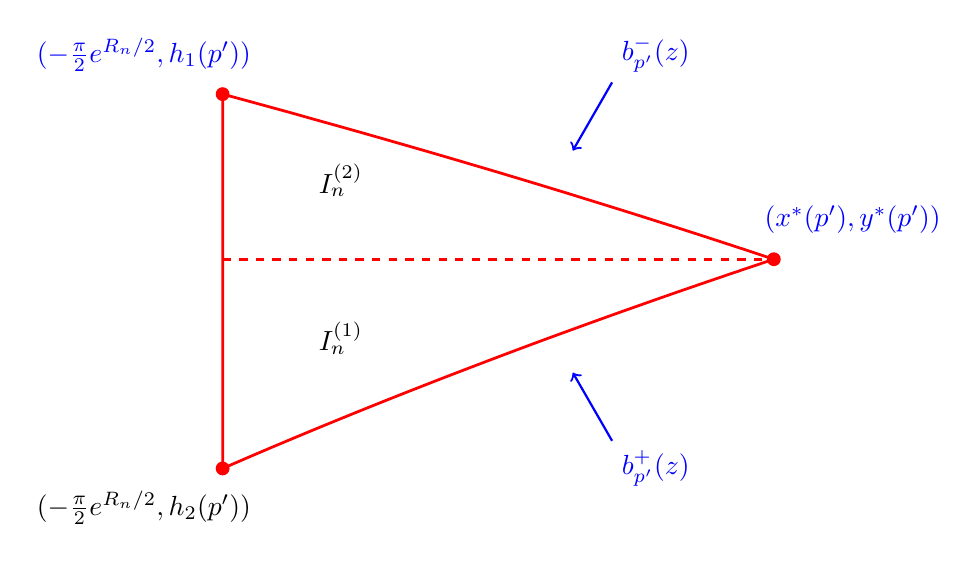
\begin{tikzpicture}[scale=5]

%%%%%%%%%%%%%%%%%%%%%%%%%%%%%%%%%%%%%%%%%%%%%%%%%%%%%%%%%%%%%%%%%%%%%%%%%%%%%%%%%%%%%%%%%%%%%%%%%%%
%																								  %
%	Shows the area T_{\Pcal \Delta \Pcal_n} when h_1(p^\prime) > h_2(p^\prime) > h(y)			  %
%																								  %
%%%%%%%%%%%%%%%%%%%%%%%%%%%%%%%%%%%%%%%%%%%%%%%%%%%%%%%%%%%%%%%%%%%%%%%%%%%%%%%%%%%%%%%%%%%%%%%%%%%

	%Define the coordinates 
	%p = (\u,\v) and p^\prime = (\uu, \vv)
	%Box \Rcal_n has width 2\r and height \t
	\pgfmathsetmacro{\u}{0}
	\pgfmathsetmacro{\v}{1}
	\pgfmathsetmacro{\uu}{1.4}
	\pgfmathsetmacro{\vv}{0.2}
	\pgfmathsetmacro{\r}{6}
	\pgfmathsetmacro{\t}{4}
    
    %Define x^\ast(p^\prime) and y^\ast(p^\prime)
    \pgfmathsetmacro{\uuast}{\uu-\r}
    \pgfmathsetmacro{\vvast}{2*ln(\r)-\vv}
    
    %Define intersection left black and shifted blue curve
    \pgfmathsetmacro{\vast}{2*ln((2*\r - \uu)/(exp(\v/2) + exp(\vv/2)))}
    \pgfmathsetmacro{\uast}{(\uu - 2*\r)/(1 + exp((\vv - \v)/2))}    
   
    %Define h_1(p) = h_2(p)
    \pgfmathsetmacro{\hp}{2*ln(\r-\u)-\v}
    
    %Define h_1(p^\prime) and h_2(p^\prime)
    \pgfmathsetmacro{\hh}{2*ln(\uu+\r)-\vv}
    \pgfmathsetmacro{\hhh}{2*ln(\r-\uu)-\vv}
    
    %Draw the boundary left black, left blue and shifted right blue line
	\draw[red,line width=1pt] 
		plot[domain=\uuast:-\r,smooth,variable=\x,red] (\x, {2*ln(\x+(2*\r-\uu))-\vv}) 
		-- 
		(-\r,\hh)
		-- 
		plot[domain=-\r:\uuast,smooth,variable=\x,red] (\x, {2*ln(\uu-\x)-\vv});
	
	\pgfmathsetmacro{\top}{2*ln(\uu-\uast)-\vv}
	
	\draw[red, dashed,line width=1pt] (-\r,\vvast) -- (\uuast,\vvast);

    \draw node at (-\r-0.2,\hh+0.1) {\color{blue}$(-\frac{\pi}{2} e^{R_n/2}, h_1(p^\prime))$};
    \draw node at (-\r-0.2,\hhh-0.1) {$(-\frac{\pi}{2} e^{R_n/2}, h_2(p^\prime))$};
    \draw node at (\uuast+0.2,\vvast+0.1) {\color{blue}$(x^\ast(p^\prime), y^\ast(p^\prime))$};
    
    \draw node at (-\r+0.3,\vvast+0.2) {$I_n^{(2)}$};
    \draw node at (-\r+0.3,\vvast-0.2) {$I_n^{(1)}$};
    
    \draw node (f2) at (\uuast-0.3,\hh+0.1) {\color{blue}$b_{p^\prime}^-(z)$};
    \draw node (f3) at (\uuast-0.3,\hhh) {\color{blue}$b_{p^\prime}^+(z)$};
    \path (f2)+(230:0.35) node (f2_arrow) {};
    \path (f3)+(130:0.35) node (f3_arrow) {};
    \draw[->,thick,blue] (f2.south west) -- (f2_arrow);
    \draw[->,thick,blue] (f3.north west) -- (f3_arrow);

	\draw node[red, fill, circle, inner sep=0pt, minimum size=5pt] at (-\r,\hhh) {};
	\draw node[red, fill, circle, inner sep=0pt, minimum size=5pt] at (-\r,\hh) {};
	\draw node[red, fill, circle, inner sep=0pt, minimum size=5pt] at (\uuast,\vvast) {};

\end{tikzpicture}\\
\vspace{20pt}
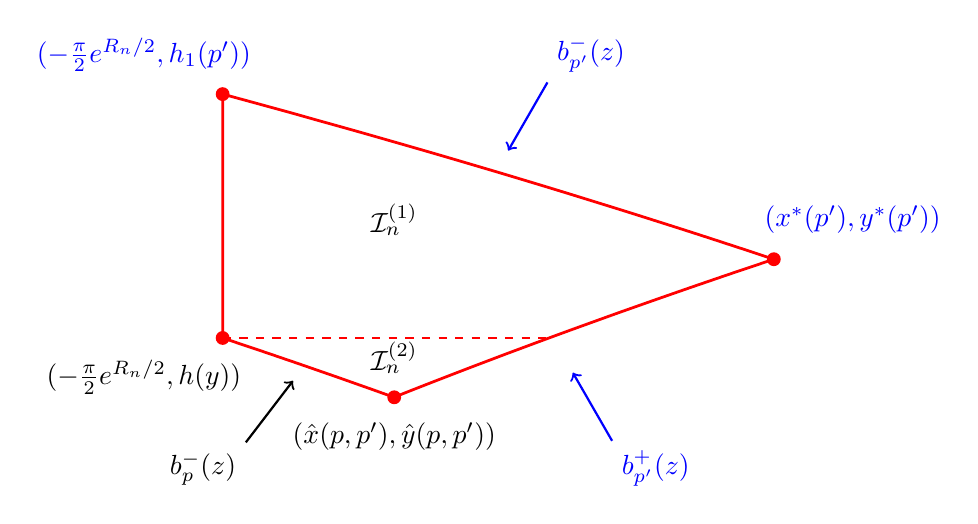
\begin{tikzpicture}[scale=5]
	%Define the coordinates 
	%p = (\u,\v) and p^\prime = (\uu, \vv)
	%Box \Rcal_n has width 2\r and height \t
	\pgfmathsetmacro{\u}{0}
	\pgfmathsetmacro{\v}{1}
	\pgfmathsetmacro{\uu}{1.4}
	\pgfmathsetmacro{\vv}{0.8}
	\pgfmathsetmacro{\r}{6}
	\pgfmathsetmacro{\t}{4}
    
    %Define x^\ast(p^\prime) and y^\ast(p^\prime)
    \pgfmathsetmacro{\uuast}{\uu-\r}
    \pgfmathsetmacro{\vvast}{2*ln(\r)-\vv}
    
    %Define intersection left black and shifted blue curve
    \pgfmathsetmacro{\vast}{2*ln((2*\r - \uu)/(exp(\v/2) + exp(\vv/2)))}
    \pgfmathsetmacro{\uast}{(\uu - 2*\r)/(1 + exp((\vv - \v)/2))}    
   
    %Define h_1(p) = h_2(p)
    \pgfmathsetmacro{\hp}{2*ln(\r-\u)-\v}
    
    %Define h_1(p^\prime) and h_2(p^\prime)
    \pgfmathsetmacro{\hh}{2*ln(\uu+\r)-\vv}
    \pgfmathsetmacro{\hhh}{2*ln(\r-\uu)-\vv}
    
    %Draw the boundary left black, left blue and shifted right blue line
	\draw[red,line width=1pt] 
		plot[domain=\uuast:\uast,smooth,variable=\x,red] (\x, {2*ln(\x+(2*\r-\uu))-\vv}) 
		-- 
		plot[domain=\uast:-\r,smooth,variable=\x,red] (\x, {2*ln(-\x)-\v})
		-- 
		(-\r,\hh)
		-- 
		plot[domain=-\r:\uuast,smooth,variable=\x,red] (\x, {2*ln(\uu-\x)-\vv});
	
	\pgfmathsetmacro{\rb}{\uu + exp((\vv+\hp)/2) -2*\r}
	

	%\draw[red,dashed,line width=1pt] (\uast,\vast) -- (\uast,\hp);
	\draw[red,dashed,line width=1pt] (-\r,\hp) -- (\rb,\hp);

    \draw node at (-\r-0.2,\hh+0.1) {\color{blue}$(-\frac{\pi}{2} e^{R_n/2}, h_1(p^\prime))$};
    \draw node at (-\r-0.2,\hp-0.1) {$(-\frac{\pi}{2} e^{R_n/2}, h(y))$};
    \draw node at (\uuast+0.2,\vvast+0.1) {\color{blue}$(x^\ast(p^\prime), y^\ast(p^\prime))$};
    \draw node at (\uast,\vast-0.1) {$(\hat{x}(p,p^\prime), \hat{y}(p, p^\prime))$};
    
    \draw node at (\uast,\vvast+0.1) {$\mathcal{I}_n^{(1)}$};
    \draw node at (\uast,\hp-0.05) {$\mathcal{I}_n^{(2)}$};
    %\draw node at (\uast+0.1,\hp-0.05) {$\mathcal{I}_n^{(3)}$};
    
    \draw node (f1) at (-\r-0.05,\hhh) {$b_p^-(z)$};
    \draw node (f2) at (\uast+0.5,\hh+0.1) {\color{blue}$b_{p^\prime}^-(z)$};
    \draw node (f3) at (\uuast-0.3,\hhh) {\color{blue}$b_{p^\prime}^+(z)$};
    \path (f1)+(45:0.35) node (f1_arrow) {};
    \path (f2)+(230:0.35) node (f2_arrow) {};
    \path (f3)+(130:0.35) node (f3_arrow) {};
    \draw[->,thick] (f1.north east) -- (f1_arrow);
    \draw[->,thick,blue] (f2.south west) -- (f2_arrow);
    \draw[->,thick,blue] (f3.north west) -- (f3_arrow);

	\draw node[red, fill, circle, inner sep=0pt, minimum size=5pt] at (-\r,\hp) {};
	\draw node[red, fill, circle, inner sep=0pt, minimum size=5pt] at (-\r,\hh) {};
	\draw node[red, fill, circle, inner sep=0pt, minimum size=5pt] at (\uuast,\vvast) {};
	\draw node[red, fill, circle, inner sep=0pt, minimum size=5pt] at (\uast,\vast) {};

\end{tikzpicture}\\
\vspace{20pt}
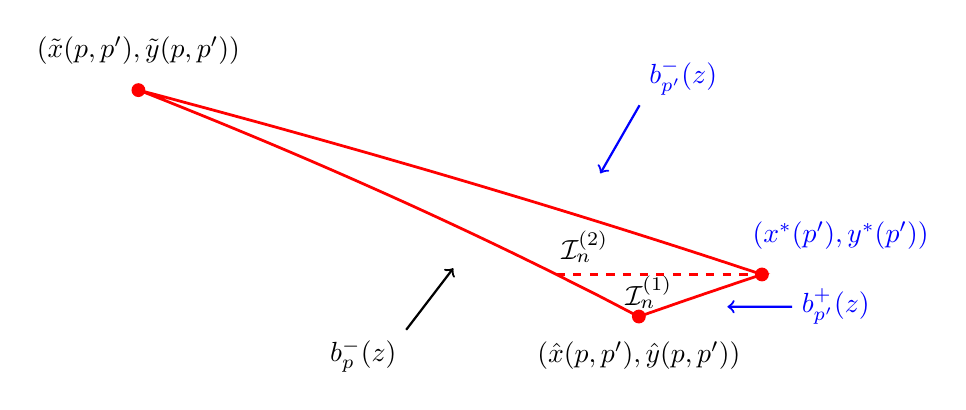
\begin{tikzpicture}[scale=5]

%%%%%%%%%%%%%%%%%%%%%%%%%%%%%%%%%%%%%%%%%%%%%%%%%%%%%%%%%%%%%%%%%%%%%%%%%%%%%%%%%%%%%%%%%%%%%%%%%%%
%																								  %
%	Shows the area T_{\Pcal \Delta \Pcal_n} when h(y) > h_1(p^\prime)							  %
%																								  %
%%%%%%%%%%%%%%%%%%%%%%%%%%%%%%%%%%%%%%%%%%%%%%%%%%%%%%%%%%%%%%%%%%%%%%%%%%%%%%%%%%%%%%%%%%%%%%%%%%%

	%Define the coordinates 
	%p = (\u,\v) and p^\prime = (\uu, \vv)
	%Box \Rcal_n has width 2\r and height \t
	\pgfmathsetmacro{\u}{0}
	\pgfmathsetmacro{\v}{1}
	\pgfmathsetmacro{\uu}{2.5}
	\pgfmathsetmacro{\vv}{1.8}
	\pgfmathsetmacro{\r}{6}
	\pgfmathsetmacro{\t}{4}
    
    %Define x^\ast(p^\prime) and y^\ast(p^\prime)
    \pgfmathsetmacro{\uuast}{\uu-\r}
    \pgfmathsetmacro{\vvast}{2*ln(\r)-\vv}
    
    %Define intersection left black and shifted blue curve
    \pgfmathsetmacro{\vast}{2*ln((2*\r - \uu)/(exp(\v/2) + exp(\vv/2)))}
    \pgfmathsetmacro{\uast}{(\uu - 2*\r)/(1 + exp((\vv - \v)/2))}    
    
    %Define intersection left black and left blue curve
    \pgfmathsetmacro{\utilde}{\uu/(1-exp((\vv-\v)/2))} 
    \pgfmathsetmacro{\vtilde}{2*ln(\uu-\utilde)-\vv}
   
    %Define h_1(p) = h_2(p)
    \pgfmathsetmacro{\hp}{2*ln(\r-\u)-\v}
    
    %Define h_1(p^\prime) and h_2(p^\prime)
    \pgfmathsetmacro{\hh}{2*ln(\uu+\r)-\vv}
    \pgfmathsetmacro{\hhh}{2*ln(\r-\uu)-\vv}
    
    %Draw the boundary left black, left blue and shifted right blue line
	\draw[red,line width=1pt] 
		plot[domain=\utilde:\uuast,smooth,variable=\x,red] (\x, {2*ln(\uu-\x)-\vv})
		--
		plot[domain=\uuast:\uast,smooth,variable=\x,red] (\x, {2*ln(\x+(2*\r-\uu))-\vv})
		--
		plot[domain=\uast:\utilde,smooth,variable=\x,red] (\x, {2*ln(-\x)-\v}); 
	
	%Calculate intersection point
	\pgfmathsetmacro{\i}{-exp((\v+\vvast)/2)}
	\draw[red, dashed,line width=1pt] (\i,\vvast) -- (\uuast,\vvast);

    \draw node at (\utilde,\vtilde+0.1) {\color{black}$(\tilde{x}(p,p^\prime), \tilde{y}(p,p^\prime))$};
    \draw node at (\uast,\vast-0.1) {$(\hat{x}(p,p^\prime), \hat{y}(p,p^\prime))$};
    \draw node at (\uuast+0.2,\vvast+0.1) {\color{blue}$(x^\ast(p^\prime), y^\ast(p^\prime))$};
   
    \draw node at (\uuast-0.45,\vvast+0.07) {$\mathcal{I}_n^{(2)}$};
    \draw node at (\uast+0.025,\vvast-0.045) {$\mathcal{I}_n^{(1)}$};
   
    \draw node (f1) at (\uast-0.7,\vast-0.1) {\color{black}$b_{p}^-(z)$};
    \draw node (f2) at (\uuast-0.2,\vvast+0.5) {\color{blue}$b_{p^\prime}^-(z)$};
    \draw node (f3) at (\uast+0.5,\vast+0.025) {\color{blue}$b_{p^\prime}^+(z)$};
    \path (f1)+(45:0.35) node (f1_arrow) {};
    \path (f2)+(230:0.35) node (f2_arrow) {};
    \path (f3)+(180:0.3) node (f3_arrow) {};
	\draw[->,thick] (f1.north east) -- (f1_arrow);
    \draw[->,thick,blue] (f2.south west) -- (f2_arrow);
    \draw[->,thick,blue] (f3.west) -- (f3_arrow);
%
	\draw node[red, fill, circle, inner sep=0pt, minimum size=5pt] at (\utilde,\vtilde) {};
	\draw node[red, fill, circle, inner sep=0pt, minimum size=5pt] at (\uast,\vast) {};
	\draw node[red, fill, circle, inner sep=0pt, minimum size=5pt] at (\uuast,\vvast) {};

\end{tikzpicture}
\caption{The different shapes of $\mathcal{T}_{\Pcal \Delta \Pcal_n}(p,p_1)$ depending on the regime to which $p_1$ belongs. The top figure is for $p_1 \in B_n^{(1)}$, the middle for $p_1 \in B_n^{(2)}$ and the bottom one for $p_1 \in B_n^{(3)}$.}
\label{fig:shapes_triangle_mismatches}
\end{figure}

\paragraph{Regime 1: $0 \le y_1 \le y - 2\log(I_n/(I_n-x_1))$}

In this case the integral over $p_2$ splits into two parts
\begin{align*}
	\mathcal{I}_n^{(1)}(p_1) &:= \int_{h_2(p_1)}^{y^\ast(p_1)} \int_{-I_n}^{x_1 + e^{(y_1+y_2)/2}-2I_n} e^{-\alpha y_2}
		\dd x_2 \dd y_2\\
	\mathcal{I}_n^{(2)}(p_1) &:= \int_{y^\ast(p_1)}^{h_1(p_1)} \int_{x^\ast(p_1)}^{x_1 - e^{(y_1+y_2)/2}} e^{-\alpha y_2}
		\dd x_2 \dd y_2.
\end{align*}

We first compute $\mathcal{I}_n^{(1)}$.
\begin{align*}
	\mathcal{I}_n^{(1)}(p_1) &= \int_{h_2(p_1)}^{y^\ast(p_1)} \left(x_1 + e^{(y_1+y_2)/2} - I_n\right) e^{-\alpha y_2} 
		\dd x_2 \dd y_2\\
	&\le e^{y_1/2} \int_{h_2(p_1)}^{y^\ast(p_1)} e^{-(\alpha-\frac{1}{2}) y_2} \dd y_2\\
	&= \frac{2 e^{y_1/2}}{2\alpha - 1} \left(e^{-(\alpha-\frac{1}{2})h_2(p_1)} - e^{-(\alpha-\frac{1}{2})y^\ast(p_1)}
		\right) \\
	&= \frac{2 e^{\alpha y_1}}{2\alpha - 1} I_n^{-(2\alpha -1)}\left(\left(1 - \frac{x_1}{I_n}\right)^{-(2\alpha - 1)}-1\right)\\
	&= \bigO{I_n^{-2\alpha} x_1 e^{\alpha y_1}},
\end{align*}
where we used that $x^\prime \le e^{(y+y_1)/2} = \smallO{I_n}$ for all $y_1\le y$ and $y \in \Kcal_{\varepsilon}(k_n)$ so that
\[
	\left(\left(1 - \frac{x_1}{I_n}\right)^{-(2\alpha - 1)}-1\right) = \bigO{\frac{x^\prime}{I_n}} \quad 
	\text{as } n \to \infty.
\]

For $\mathcal{I}_n^{(2)}(p_1)$ we have
\begin{align*}
	\mathcal{I}_n^{(2)}(p_1) &= \int_{y^\ast(p_1)}^{h_1(p_1)} \left(I_n + x_1 - e^{(y_1+y_2)}\right) e^{-\alpha y_2}
		\dd x_2 \dd y_2\\
	&\le 2 I_n \int_{y^\ast(p_1)}^{h_1(p_1)} e^{-\alpha y_2} \dd x_2 \dd y_2\\
	&= \frac{2}{\alpha} I_n \left(I_n^{-2\alpha}e^{\alpha y_1} - \left(I_n + x_1\right)^{-2\alpha} e^{-\alpha y_1}\right)\\
	&= \bigO{I_n^{-2\alpha} x_1 e^{\alpha y_1}} = \bigO{I_n^{-(2\alpha - 1)} e^{\alpha y_1}}.
\end{align*}

We conclude that for $p_1 \in B_n^{(1)}$:
\[
	\mu_{\alpha, \nu}\left(\mathcal{T}_{\Pcal \Delta \Pcal_n}(p,p_1)\right) = \bigO{I_n^{-2\alpha} x_1 e^{\alpha y_1}},
\]
which establishes the first part of \eqref{eq:mu_triangle_diff}.

\paragraph{Regime 2: $y - 2\log(I_n/(I_n-x_1)) < y_1 \le y + 2 \log\left(1 + \frac{x_1}{I_n}\right)$}

Here we split the integration into three parts (see Figure~\ref{fig:shapes_triangle_mismatches}). Recall that $x^\ast(p,p_1) = x_1 - I_n$. Then, for the first part we have
\begin{align*}
	\mathcal{I}_n^{(1)}(p,p_1) &\le \int_{h(y)}^{h_1(p_1)} \int_{-I_n}^{x^\ast(p,p_1)} f_{\alpha,\nu}(x_2, y_2) 
		\dd x_2 \dd y_2\\
	&= \bigO{x_1 \left(e^{-\alpha h(y)} - e^{-\alpha h_1(p_1)}\right)}\\
	&= \bigO{x_1 I_n^{-2\alpha}\left(e^{\alpha y} - e^{\alpha y_1}\left(1 + \frac{x_1}{I_n}\right)^{-2\alpha}\right)}\\
	&= \bigO{I_n^{-2\alpha} x_1 e^{\alpha y_1}\left(\left(1 - \frac{x_1}{I_n}\right)^{-2\alpha} 
		- \left(1 + \frac{x_1}{I_n}\right)^{-2\alpha}\right)}\\
	&= \bigO{I_n^{-2\alpha} x_1 e^{\alpha y_1}} = \bigO{I_n^{-(2\alpha - 1)} e^{\alpha y}}, 
\end{align*}
were we used that $y \le y_1 + 2\log(I_n/(I_n-x_1))$ for $p_1 \in B_n^{(2)}$ for the third line and 
\[
	\left(1 - \frac{x_1}{I_n}\right)^{-2\alpha} - \left(1 + \frac{x_1}{I_n}\right)^{-2\alpha}
	= \bigO{\frac{x_1}{I_n}} = \bigO{1},
\]
for the last line.

For the second part we first compute that 
\begin{align*}
	x_1 + e^{(y_1+y_2)/2} - 2 I_n + e^{(y + y_2)/2} &\le \left(e^{y/2} + e^{y_1/2}\right)e^{y_2/2}\\
	&\le e^{y/2}\left(1 + \frac{I_n}{I_n - e^y}\right)e^{y_2/2} = \bigO{e^{(y+y_2)/2}},
\end{align*}
since $y \in \Kcal_{\varepsilon}(k_n)$ and $k_n = \smallO{\sqrt{n}}$, so that $e^y = \smallO{n} = \smallO{I_n}$. 
Then we have
\begin{align*}
	\mathcal{I}_n^{(2)} &= \int_{\hat{y}(p,p_1)}^{h(y)} \int_{-e^{(y + y_2)/2}}^{x_1 + e^{(y+y_1)/2} - 2 I_n} 
		f_{\alpha,\nu}(x_2, y_2) \dd x_2 \dd y_2\\
	&= \bigO{e^{y/2} \int_{\hat{y}(p,p_1)}^{h(y)} e^{-(\alpha -\frac{1}{2}) y_2} \dd y_2}\\
	&= \bigO{e^{y/2} \left(e^{-(\alpha -\frac{1}{2}) \hat{y}(p,p_1)} - e^{-(\alpha -\frac{1}{2}) h(y)}\right)}\\
	&= \bigO{e^{y/2} \left(\left(\frac{2I_n - x_1}{e^{y/2} + e^{y_1/2}}\right)^{-(2\alpha-1)} 
		- I_n^{-(2\alpha-1)} e^{(\alpha -\frac{1}{2}) y}\right)}\\
	&= \bigO{I_n^{-(2\alpha-1)} e^{\alpha y}},
\end{align*}
where for the last line we first used that $(2I_n - x_1)^{-(2\alpha-1)} \le I_n^{-(2\alpha-1)}$ and then
\[
	\left(\left(e^{y/2} + e^{y_1/2}\right)^{2\alpha-1}- e^{(\alpha -\frac{1}{2}) y}\right)
	\le e^{(\alpha -\frac{1}{2}) y}\left(\left(1 + \sqrt{1+\frac{x_1}{I_n}} \, \right)^{2\alpha - 1} - 1\right)
	= \bigO{e^{(\alpha -\frac{1}{2}) y}}.
\]

It then follows that for $p_1 \in B_n^{(2)}$
\[
	\mu_{\alpha, \nu}\left(\mathcal{T}_{\Pcal \Delta \Pcal_n}(p,p_1)\right) = \bigO{I_n^{-(2\alpha-1)} e^{\alpha y}}.
\]

\paragraph{Regime III $\bm{p_1 \in B_n^{(3)}}$:}

\begin{align*}
	\mathcal{I}_n^{(1)} &= \int_{y^\ast}^{\tilde{y}} \int_{-e^{(y+y_2)/2}}^{x_1-e^{(y_1+y_2)/2}} f_{\alpha, \nu}(x_2,y_2)
		\dd x_2 \dd y_2\\
	&= \bigO{\int_{y^\ast}^{\tilde{y}} x_1 e^{-\alpha y_2} - \left(e^{y_1/2} - e^{y/2}\right)e^{-(\alpha - \frac{1}{2})y_2}
		\dd y_2}\\
	&= \bigO{x_1 \int_{y^\ast}^{\tilde{y}}  e^{-\alpha y_2} \dd y_2}.
\end{align*}

Now 
\begin{align*}
	\int_{y^\ast}^{\tilde{y}}  e^{-\alpha y_2} \dd y_2 
	&= \frac{1}{\alpha}\left(e^{-\alpha y^\ast} - e^{-\alpha \tilde{y}}\right) 
		= \frac{1}{\alpha}\left(I_n^{-2\alpha} e^{\alpha y_1} 
		- \left(\frac{x_1}{e^{y_1/2} - e^{y/2}}\right)^{-2\alpha}\right) \\
	&= \frac{I_n^{-2\alpha} e^{\alpha y_1}}{\alpha}\left(1 - \left(1 - e^{(y - y_1)/2}\right)^{2\alpha}
		\left(\frac{x_1}{I_n}\right)^{-2\alpha}\right) = \bigO{I_n^{-2\alpha} e^{\alpha y_1}},
\end{align*}
and hence we have
\[
	\mathcal{I}_n^{(1)} = \bigO{I_n^{-2\alpha} x_1 e^{\alpha y_1}}.
\]

For the second integral we have
\begin{align*}
	\mathcal{I}_n^{(2)} &= \int_{\hat{y}}^{y^\ast} \int_{-e^{(y+y_2)/2}}^{e^{(y_1 + y_2)/2} + x_1 - 2I_n} 
		f_{\alpha, \nu}(x_2,y_2)\dd x_2 \dd y_2\\
	&= \bigO{\int_{\hat{y}}^{y^\ast} \left(e^{y/2} + e^{y_1/2}\right)e^{-(\alpha - \frac{1}{2})y_2} \dd y_2}\\
	&= \bigO{ e^{y_1/2} \int_{\hat{y}}^{y^\ast}e^{-(\alpha - \frac{1}{2})y_2} \dd y_2}.
\end{align*}

For the integral we have
\begin{align*}
	\int_{\hat{y}}^{y^\ast}e^{-(\alpha - \frac{1}{2})y_2} \dd y_2
	&= \frac{2}{2\alpha - 1} \left(e^{-(\alpha - \frac{1}{2})\hat{y}} - e^{-(\alpha - \frac{1}{2})y^\ast}\right)\\
	&= \frac{2}{2\alpha - 1}\left(\left(\frac{2I_n - x_1}{e^{y/2} + e^{y_1/2}}\right)^{-(2\alpha - 1)} 
		- I_n^{-(2\alpha - 1)} e^{-(\alpha - \frac{1}{2})y_1}\right)\\
	&= \bigO{I_n^{-2\alpha} x_1 e^{-(\alpha - \frac{1}{2})y_1}}
\end{align*}
so that
\[
	\mathcal{I}_n^{(2)} = \bigO{I_n^{-(2\alpha - 1)} e^{(1-\alpha)y_1}} = \bigO{I_n^{-2\alpha} x_1 e^{\alpha y}}
\]
and hence for $p_1 \in B_n^{(3)}$
\[
	\mu_{\alpha, \nu}\left(\mathcal{T}_{\Pcal \Delta \Pcal_n}(p,p_1)\right) = \bigO{I_n^{-2\alpha} x_1 e^{\alpha y}}
	= \bigO{I_n^{-(2\alpha - 1)} e^{\alpha y}}.
\]

\subsubsection*{Integration over $p_1$}



We now proceed with the second part of the computation leading to \eqref{eq:clustering_error_T_main}. Here we will integrate $\mu_{\alpha, \nu}(\mathcal{T}_{\Pcal \Delta \Pcal_n})(p,p_1)$ over the region $B_n := B_n^{(1)} \cup B_n^{(2)} \cup B_n^{(3)}$, see Figure~\ref{fig:comparing_triangles_B_areas}. Let us first identify the boundaries of these areas. 

The area $B_n^{(1)}$ is bounded from above by the line given by the equation
\[
	y_1 = y - 2\log\left(\frac{I_n}{I_n - x_1}\right).
\]
Solving this for $x_1$ yields $x_1 = I_n\left(1 - e^{(y_1-y)/2}\right)$ and hence the area $B_n^{(1)}$ is given by
\[
	B_n^{(1)} = \left\{(x_1, y_1) \, : \, 0 \le y_1 \le y, \quad 0 \le x_1 \le I_n\left(1 - e^{(y_1-y)/2}\right) \wedge e^{(y + y_1)/2} \right\}.
\]

In a similar way we have that $B_n^{(2)}$ is bounded from above by line
\[
	y_1 = y + 2\log\left(\frac{I_n}{I_n + x_1}\right),
\]
which yields $x_1 = I_n\left(e^{(y_1 - y)/2} - 1\right)$. The lower red boundary is the upper boundary of $B_n^{(2)}$ and hence we have
\[
	B_n^{(2)} = \left\{(x_1, y_1) \, : \, h_\ast(y) \le y_1 \le h^\ast(y), \,\, I_n\left(1 - e^{(y_1-y)/2}\right) \vee 
	I_n\left(e^{(y_1 - y)/2} - 1\right) \le x_1 \le e^{(y + y_1)/2} \right\}.
\]

We continue is the same way to obtain for $B_n^{(3)}$
\[
	B_n^{(3)} = \left\{(x_1, y_1) \, : \, y \le y_1 \le R_n, \,\,
	I_n\left(1 - e^{(y - y_1)/2}\right) \le x_1 \le I_n\left(e^{(y_1 - y)/2} - 1\right) \wedge e^{(y + y_1)/2} \wedge I_n \right\}.
\]

We these characterizations of the areas we now integrate $\mu_{\alpha, \nu}(\mathcal{T}_{\Pcal \Delta \Pcal_n})(p,p_1)$ over $B_n$, splitting the computations over the three different areas.

\paragraph{$\bm{p_1 \in B_n^{(1)}}:$}

We use that $I_n\left(1 - e^{(y_1-y)/2}\right) \wedge e^{(y + y_1)/2} \le I_n\left(1 - e^{(y_1-y)/2}\right)$ so that
\begin{align*}
	&\hspace{-30pt}\int_{B_n^{(1)}} \mu_{\alpha, \nu}\left(\mathcal{T}_{\Pcal \Delta \Pcal_n}(p,p_1)\right) 
		f_{\alpha,\nu}(x_1,y_1)	\dd x_1 \dd y_1 \\
	&\le  \int_0^y \int_0^{I_n(1-e^{(y_1-y)/2})} \mu_{\alpha, \nu}\left(\mathcal{T}_{\Pcal \Delta \Pcal_n}(p,p_1)\right) 
		f_{\alpha,\nu}(x_1,y_1) \dd x_1 \dd y_1\\
	&= \bigO{ I_n^{-2\alpha} \int_0^y \int_0^{e^{(y+y_1)/2}}  x_1 \dd x_1 \dd y_1 }\\
	&= \bigO{I_n^{-(2\alpha-1)} \int_0^y \left(1 - e^{(y_1-y)/2}\right)^2 \dd y_1} \\
	&= \bigO{I_n^{-(2\alpha - 1)} y} = \bigO{y n^{-(2\alpha - 1)}}.
\end{align*} 

\paragraph{$\bm{p_1 \in B_n^{(2)}}:$}

We will show that
\begin{equation}\label{eq:mu_triangle_diff_2}
	\mu_{\alpha, \nu}(B_n^{(2)}) = \bigO{I_n^{-1} e^{(2-\alpha)y}},
\end{equation}
which together with \eqref{eq:mu_triangle_diff} yields
\begin{align*}
	\int_{B_n^{(2)}} \mu_{\alpha, \nu}\left(\mathcal{T}_{\Pcal \Delta \Pcal_n}(p,p_1)\right) 
		f_{\alpha,\nu}(x_1,y_1)	\dd x_1 \dd y_1
	&= \bigO{\mu_{\alpha, \nu}(B_n^{(2)}) I_n^{-(2\alpha - 1)} e^{\alpha y}}\\
	&= \bigO{I_n^{-2\alpha} e^{2y}}.
\end{align*}

The integration is split into two parts determined by $I_n\left(1 - e^{(y_1-y)/2}\right) \vee 
	I_n\left(e^{(y_1 - y)/2} - 1\right)$:
\begin{align*}
	\mu_{\alpha, \nu}(B_n^{(3)}) &= \int_{h_\ast(y)}^{y} \int_{I_n(1-e^{(y_1-y)/2})}^{e^{(y + y_1)/2}} 
		f_{\alpha,\nu}(x_1,y_1) \dd x_1 \dd y_1\\
	&\hspace{10pt} + \int_y^{h^\ast(y)} \int_{I_n(e^{(y_1-y)/2}-1)}^{e^{(y + y_1)/2}} 
		f_{\alpha,\nu}(x_1,y_1) \dd x_1 \dd y_1.
\end{align*}

For the first integral we use that $e^{(y + y_1)/2} - I_n(1-e^{(y_1-y)/2}) \le e^{y_1/2}\left(e^{y/2} + e^{-y/2}\right)$ to obtain
\begin{align*}
	&\hspace{-30pt}\int_{h_\ast(y)}^{y} \int_{I_n(1-e^{(y_1-y)/2})}^{e^{(y + y_1)/2}} f_{\alpha,\nu}(x_1,y_1) 
		\dd x_1 \dd y_1\\
	&= \bigO{e^{y/2} \int_{h_\ast(y)}^{y} e^{-(\alpha - \frac{1}{2})y_1} \dd y_1}\\
	&= \bigO{e^{y/2}\left(e^{-(\alpha - \frac{1}{2})y} - e^{-(\alpha - \frac{1}{2})y} 
		\left(\frac{I_n}{I_n + e^y}\right)^{-(2\alpha - 1)}\right)}\\
	&= \bigO{I_n^{-1} e^{(2-\alpha)y}}.
\end{align*}
For the second integral note that $e^{(y + y_1)/2} - I_n(e^{(y_1-y)/2}-1) \le e^{(y + y_1)/2}$ and hence
\begin{align*}
	&\hspace{-30pt}\int_y^{h^\ast(y)} \int_{I_n(e^{(y_1-y)/2}-1)}^{e^{(y + y_1)/2}} f_{\alpha,\nu}(x_1,y_1) 
		\dd x_1 \dd y_1\\
	&= \bigO{e^{y/2} \int_y^{h^\ast(y)} e^{-(\alpha - \frac{1}{2})y_1} \dd y_1}\\
	&= \bigO{e^{y/2} \left(e^{-(\alpha - \frac{1}{2})y} - e^{-(\alpha - \frac{1}{2})y}
		\left(\frac{I_n}{I_n - e^y}\right)^{-(2\alpha - 1)}\right)}\\
	&= \bigO{I_n^{-1} e^{(2-\alpha)y}},
\end{align*}
so that \eqref{eq:mu_triangle_diff_2} follows.

\paragraph{$\bm{p_1 \in B_n^{(3)}}:$}

For this area we show that 
\begin{equation}\label{eq:mu_triangle_diff_3}
	\mu_{\alpha, \nu}(B_n^{(3)}) = \bigO{e^{(1-\alpha)y}}
\end{equation} 
so that
\begin{align*}
	\int_{B_n^{(3)}} \mu_{\alpha, \nu}\left(\mathcal{T}_{\Pcal \Delta \Pcal_n}(p,p_1)\right) 
		f_{\alpha,\nu}(x_1,y_1)	\dd x_1 \dd y_1
	&= \bigO{\mu_{\alpha, \nu}(B_n^{(2)}) I_n^{-(2\alpha - 1)} e^{\alpha y}}\\
	&= \bigO{I_n^{-(2\alpha-1)} e^{y}}.
\end{align*}

Here the integral is split into three parts:
\begin{align*}
	\mu_{\alpha, \nu}(B_n^{(3)}) &= \int_y^{h^\ast(y)} \int_{I_n(1-e^{(y-y_1)/2})}^{I_n(e^{(y_1-y)/2}-1)}
		f_{\alpha,\nu}(x_1,y_1) \dd x_1 \dd y_1\\
	&\hspace{10pt}+ \int_{h^\ast(y)}^{h(y)} \int_{I_n(1-e^{(y-y_1)/2})}^{e^{(y+y_1)/2}}
		f_{\alpha,\nu}(x_1,y_1) \dd x_1 \dd y_1\\
	&\hspace{10pt}+ \int_{h(y)}^{R_n} \int_{I_n(1-e^{(y-y_1)/2})}^{I_n}
		f_{\alpha,\nu}(x_1,y_1) \dd x_1 \dd y_1.
\end{align*}

Let us first focus on the first integral. Since	$I_n(e^{(y_1-y)/2}-1) - I_n(1-e^{(y-y_1)/2}) \le I_n e^{(y_1-y)/2}$ we get,
using similar arguments as above
\begin{align*}
	\int_y^{h^\ast(y)} \int_{I_n(1-e^{(y-y_1)/2})}^{I_n(e^{(y_1-y)/2}-1)} f_{\alpha,\nu}(x_1,y_1) \dd x_1 \dd y_1
	&= \bigO{I_n e^{-y/2} \int_y^{h^\ast(y)} e^{-(\alpha - \frac{1}{2})y_1} \dd y_1}\\
	&= \bigO{I_n e^{-\alpha y} \left(1 - \left(\frac{I_n}{I_n - e^y}\right)^{-(2\alpha - 1)}\right)}\\
	&= \bigO{e^{(1-\alpha)y}}.
\end{align*}

Proceeding to the second integral, we first note that $e^{(y+y_1)/2} - I_n(1-e^{(y-y_1)/2}) = \bigO{I_n e^{(y_1-y)/2}}$ so that similar calculations as before yield
\begin{align*}
	\int_{h^\ast(y)}^{h(y)} \int_{I_n(1-e^{(y-y_1)/2})}^{e^{(y+y_1)/2}}	f_{\alpha,\nu}(x_1,y_1) \dd x_1 \dd y_1
	&= \bigO{I_n e^{-y/2} \int_{h^\ast(y)}^{h(y)} e^{-(\alpha - \frac{1}{2})y_1} \dd y_1}
		= \bigO{e^{(1-\alpha)y}}.
\end{align*}



\end{proof}